\documentclass[journal]{IEEEtai}

\usepackage{amsmath,amssymb,mathtools,amsthm}
\usepackage{bm}
\usepackage{multirow}
\usepackage{booktabs}
\usepackage{algorithm}
\usepackage{algorithmic}
\usepackage{graphicx}
\usepackage{enumitem}
\usepackage{subfigure}
\usepackage[caption=false,font=footnotesize]{subfig}
\usepackage[colorlinks,urlcolor=blue,linkcolor=blue,citecolor=blue]{hyperref}

% Custom macros
\DeclareMathOperator*{\argmin}{arg\,min}
\newcommand{\TSP}{\textsc{TSP}}
\newcommand{\CVRP}{\textsc{CVRP}}
\newcommand{\ACO}{\textsc{ACO}}
\newcommand{\DyNACO}{\textsc{DyNACO}}
\newcommand{\DyNACS}{\textsc{DyNACS}}
\newcommand{\MMAS}{\textsc{MMAS}}
\newcommand{\VRP}{\textsc{VRP}}

\newtheorem{theorem}{Theorem}
\newtheorem{lemma}{Lemma}

% Populate these fields after acceptance, when supplied by IEEE.
%% \jvol{XX}
%% \jnum{XX}
%% \paper{XXXXXXX}
%% \pubyear{2026}
%% \publisheddate{Month 00, 2026}
%% \currentdate{Month 00, 2026}
%% \doiinfo{TAI.2026.XXXXXXX}

\begin{document}

\title{Generalizable Dynamic Neural Ant Colony Search for Large-Scale Routing Problems}

\author{Dat Thanh Tran, Van Khu Vu, and Yining Ma
\thanks{Manuscript received Month 00, 2026; revised Month 00, 2026.}
\thanks{Dat Thanh Tran is with the Center for AI Research, VinUniversity, Hanoi, Vietnam (e-mail: dat.tt3@vinuni.edu.vn).}
\thanks{Van Khu Vu is with the College of Engineering and Computer Science, VinUniversity, Hanoi, Vietnam (e-mail: khu.vv@vinuni.edu.vn).}
\thanks{Yining Ma is with the Laboratory for Information and Decision Systems, Massachusetts Institute of Technology, Cambridge, MA 02139 USA (e-mail: yiningma@mit.edu).}
\thanks{Corresponding author: Yining Ma.}}

\markboth{IEEE Transactions on Artificial Intelligence, Vol. 00, No. 0, Month 2026}%
{Tran \MakeLowercase{\textit{et al.}}: Dynamic Neural Ant Colony Search for Large-Scale Routing Problems}

\maketitle

\begin{abstract}
Neural guidance for Ant Colony Optimization (ACO) is usually trained as a static heatmap, but it is deployed inside an iterative search process whose pheromones and incumbent solutions evolve over time. The resulting training--inference mismatch limits search adaptivity and weakens zero-shot generalization, because a fixed neural prior learned from one distribution may become unreliable on benchmark instances with different scales and structures. We introduce \DyNACO{}, a dynamic neural ACO model that periodically observes the pheromone distribution and incumbent solution, then updates edge guidance throughout the search trajectory. State-aware guidance keeps the neural signal coupled to the evolving solver state; population-aware guidance further lets different ant groups express complementary transition biases at the same state. We introduce \DyNACS{} (Dynamic Neural Ant Colony Search), which equips the shared colony with several behavior-conditioned trajectory distributions. Different ant groups follow complementary transition priors while updating the same incumbent and pheromone process. To keep neural guidance trainable at scale, we use perturbation-based ACO with scope-restricted refinement, so neural decisions remain local enough for stable credit assignment yet still receive convergent local projection. Under a zero-shot protocol, a single model trained only on 1K-node instances achieves $1.22\%$ average gap on \TSP{} and $2.80\%$ on \CVRP{} across benchmark datasets, outperforming all state-of-the-art neural baselines under matched evaluation. On \TSP{}, \DyNACS{} scales to 100,000-node instances and often reduces total runtime compared with the unguided solver; on \CVRP{}, it consistently improves the unguided baseline with less than $1\%$ neural overhead. The results indicate that neural guidance can generalize beyond synthetic training distributions when it adapts to the solver state and preserves useful diversity in the ant population.
\end{abstract}


\begin{IEEEImpStatement}
Large routing problems arise in logistics, transportation, and network design, where practical instances often differ substantially from the synthetic distributions used to train neural solvers. Our results show that neural guidance can be integrated into an established ant colony optimizer while preserving its iterative search structure. By adapting guidance during search and maintaining complementary search behaviors, \DyNACS{} improves robustness under distribution shift while preserving the scalability of the underlying solver. More broadly, the work supports a practical direction for learning-guided optimization: neural components should read and update the internal state of classical solvers instead of producing one-shot predictions detached from the search process.
\end{IEEEImpStatement}


\begin{IEEEkeywords}
Ant colony optimization, combinatorial optimization, learning-guided optimization, neural combinatorial optimization, reinforcement learning.
\end{IEEEkeywords}

\section{Introduction}

% \IEEEPARstart{C}{ombinatorial} optimization problems (COPs) such as the Traveling Salesman Problem (\TSP{}) and the capacitated Vehicle Routing Problem (\CVRP{}) have broad applications in logistics and network design~\cite{TSPAPP}.
% As NP-hard problems, they are typically tackled with heuristics.
% Classical solvers such as LKH-3~\cite{lkhtsp, lkhcvrp} and HGS~\cite{hgs} achieve near-optimal precision through decades of engineering, while recent Machine Learning (ML) based neural combinatorial optimization (NCO)~\cite{MLCO, RL4CO,neuopt,2optlearning} has emerged as a data-driven alternative. However, end-to-end NCO models often struggle with scalability, generalization, and a lack of convergence guarantees~\cite{RL4CO}. Learning-guided optimization (LGO)~\cite{learn2branch, learn2delegate, neurolkh} bridges this gap by integrating neural signals into classical human solvers, which often achieves state-of-the-art performance by effectively combining the strengths of both paradigms~\cite{learn2delegate,deepaco,learn2seg,huang2024contrastive}.

% Among the LGO methods, learning to guide Ant Colony Optimization (ACO)~\cite{ACO, maxmin} serves as a foundational approach for steering meta-heuristics~\cite{deepaco,gtgaco}. ACO is a population-based metaheuristic where artificial ants construct solutions via probabilistic transitions biased by pheromone updates toward promising regions. In general, ACO factorizes the transition rule by combining dynamic pheromone updates with heuristic priors. While recent methods successfully learn to initialize such heuristic priors~\cite{deepaco,gfacs} or both heuristics and pheromone matrices~\cite{gtgaco}, they all share a critical flaw: they train a model to produce guidance from instance geometry \emph{only once}, yielding static heatmaps, and then deploy this fixed signal inside a full ACO loop where pheromone dynamics evolve over hundreds of iterations.
% The model never observes pheromone during training and has no mechanism to adapt to it at inference.
% This \emph{training-inference misalignment} renders the neural signal blind to search progress: it applies identical guidance regardless of whether pheromones are near-uniform (early search) or concentrated around a local optimum (late search).
% % HeatACO~\cite{heataco} confirms that under this static paradigm the model architecture is interchangeable, suggesting that the static integration strategy itself is the limiting factor.

% Motivated by this, we propose \textbf{\DyNACO{}}, a framework that shifts from \emph{static} to \emph{dynamic} neural guidance. While prior methods train the model on a single snapshot of instance geometry and freeze the output, \DyNACO{} trains its policy on the \emph{full search trajectory}: the model repeatedly observes the evolving pheromone distribution and incumbent solution, and learns to emit guidance that is useful at every stage of the search, not just at initialization. To enable this, we design a specialized module to extract representations that summarize the current optimization status. 
% We formalize this as a \emph{semi-Markov Decision Process} in which a meta-policy periodically observes search state and emits updated edge-level guidance, and we train \DyNACO{}  with a reinforcement learning algorithm.

% Another key limitation of existing neural-guided ACO methods is scalability. To make \DyNACO{} tractable at scale, we pair the policy with a perturbation-based ACO backend on a sparse $K$-nearest-neighbor graph and a \emph{scope-restricted refinement} (SRR) mechanism. Because the resulting perturbations are highly localized, our design delivers three simultaneous benefits: (1) \emph{Stable Credit Assignment}: confining refinement to the neighborhood of the policy's actions preserves the causal link between those actions and post-refinement rewards; (2) \emph{Within-Scope Convergence}: SRR exhaustively applies 2-opt moves around the perturbed edges until no further improvement, ensuring local optimality that guarantees performance; and (3) \emph{Size-Independent Scalability}: the per-ant refinement cost is reduced from $\mathcal{O}(N^2)$ to $\mathcal{O}(M \cdot K)$, making stable training feasible at the 100,000-node scale.

% Extensive experiments on TSP and CVRP demonstrate that \DyNACO{} significantly outperforms existing neural ACO baselines under matched budgets, and surpasses established classical and neural baselines, especially on real-world large-scale instances. On TSP, neural guidance actually \emph{reduces} total runtime by 23-33\% over the unguided solver, as better-targeted perturbations accelerate local-search convergence; on CVRP, neural overhead stays below 1\%, and end-to-end wall-clock overhead remains within 1-3\% at large scales, with consistent quality gains. Finally, we conduct in-depth analyses revealing the learned guidance patterns and explaining their superiority over static priors: in particular, the policy actively counteracts ACO stagnation~\cite{stagnation} by suppressing over-reinforced edges and redirecting search toward under-explored regions. Our work underscores the necessity of aligning neural training with iterative search dynamics in learning-guided optimization.

% % \noindent\textbf{Contributions.}
% Our contributions are as follows:
% (i)~we propose \DyNACO{}, the first framework for dynamic neural guidance in ACO, formulated as a semi-MDP that lets a policy inject updated guidance at regular intervals rather than committing to a single static prediction;
% (ii)~we introduce SRR, confining local search to the perturbation neighborhood to preserve credit assignment and achieve 2-opt optimality with efficiency;
% (iii)~we show that \DyNACO{} scales to 100K nodes while reducing total runtime on TSP and adding $<$1\% overhead on CVRP, with zero-shot transfer on TSPLIB and CVRPlib confirming cross-scale and cross-distribution generalization.

\IEEEPARstart{C}{ombinatorial} optimization problems (COPs), such as the Traveling Salesman Problem (\TSP{}) and the Capacitated Vehicle Routing Problem (\CVRP{}), have broad applications in logistics, transportation, and network design~\cite{TSPAPP}. As NP-hard problems, they are typically tackled by heuristic solvers. Classical solvers such as LKH-3~\cite{lkhtsp,lkhcvrp} and HGS~\cite{hgs} achieve near-optimal performance through decades of manual algorithm engineering, while recent neural combinatorial optimization (NCO) methods~\cite{MLCO,RL4CO,neuopt,2optlearning} aim to learn heuristic rules automatically from data. Despite their promise, the practical adoption of neural routing solvers remains limited by generalization. A solver trained on one distribution should remain effective when directly applied to instances with different scales, structures, and benchmark distributions. However, recent studies show that many neural routing solvers degrade sharply under zero-shot evaluation, and some even fall behind simple construction heuristics such as nearest neighbor and random insertion~\cite{nrs_survey}.

Learning-guided optimization (LGO)~\cite{learn2branch,learn2delegate,neurolkh} offers a promising path toward more reliable neural solvers by embedding learned signals into classical heuristic frameworks. Instead of replacing the entire solver with an end-to-end neural policy, LGO improves specific algorithmic components while preserving the robustness and scalability of mature solvers~\cite{learn2delegate,deepaco,learn2seg,huang2024contrastive}. Among these methods, learning to guide Ant Colony Optimization (ACO)~\cite{ACO,maxmin} is a representative direction for neural assistance in population search~\cite{deepaco,gtgaco}. ACO constructs candidate solutions through probabilistic transitions biased by heuristic priors and dynamically updated pheromones. Its population mechanism makes it naturally suitable for exploration and adaptation, but current neural ACO methods use this structure only partially.

Most existing neural ACO methods learn static edge guidance from the input instance: some initialize the heuristic prior~\cite{deepaco,gfacs}, while others learn both heuristic and pheromone-like matrices~\cite{gtgaco}. In these designs, the neural model observes instance geometry once, and the resulting heatmap remains fixed throughout the ACO search. The solver it guides is not fixed. Pheromones concentrate, incumbent solutions change, and the population gradually shifts from broad exploration toward exploitation or stagnation. A heatmap learned from a narrow source distribution may therefore become unreliable when benchmark instances induce different search trajectories.

This mismatch raises the central question for neural-guided ACO: can neural guidance be learned as a state-dependent signal that remains useful as the ACO trajectory evolves? We answer this question with \textbf{\DyNACO{}} (Dynamic Neural Ant Colony Optimization), a dynamic base model for neural ACO\@. Instead of emitting a single heatmap before search begins, \DyNACO{} learns a policy over the search trajectory. The policy periodically observes the current pheromone distribution and incumbent solution, extracts a representation of the optimization state, and emits updated guidance over candidate edges for the next search phase. We formalize this interaction as a \emph{semi-Markov Decision Process}, where each high-level policy action influences a block of low-level ACO iterations. Neural guidance thereby becomes part of the iterative solver state rather than a fixed pre-processing signal.

\DyNACO{} resolves the state mismatch, but ACO also derives strength from population search. At a macro-step, a single dynamic guidance field gives the whole colony one learned transition bias, even though different ant groups can usefully explore different continuations around the same pheromone state. We therefore introduce \textbf{\DyNACS{}} (Dynamic Neural Ant Colony Search), which gives the dynamic colony several learned search behaviors. A shared state encoder produces behavior-conditioned trajectory distributions for different ant groups. These groups sample different perturbation trajectories, contribute to the same refined candidate pool, and update the same incumbent solution and pheromone process. A learned allocation policy assigns ant mass from the current search state, allowing the colony to change its population composition as the search evolves.

The learned guidance must also remain trainable at the scales where zero-shot generalization matters. We therefore pair \DyNACO{} and \DyNACS{} with a perturbation-based ACO environment on a sparse $K$-nearest-neighbor graph. Each policy action changes a localized part of the incumbent solution, and \emph{scope-restricted refinement} (SRR) projects the resulting trajectory back to a locally consistent solution by refining only around the affected edges. This keeps rewards tied to policy actions, avoids spending refinement effort on unrelated parts of the tour, and allows the same training and inference procedure to scale to very large routing instances.

We evaluate \DyNACS{} under a strict zero-shot protocol for both \TSP{} and \CVRP{}. A single model is trained only on 1K-node synthetic instances and is then tested directly on benchmark datasets with different scales and structures, without retraining, fine-tuning, or tuning for individual instances. \DyNACS{} consistently improves the unguided backend and prior neural baselines. Further analyses show adaptive guidance beyond short-edge preference: the policy responds to the evolving pheromone landscape, suppresses over-reinforced edges when the search begins to stagnate, and maintains complementary behaviors across the ant population.

The contributions of the paper are summarized as follows:
\begin{itemize}
\item We propose \DyNACO{}, a dynamic neural ACO framework formulated as a semi-MDP, where a policy periodically observes pheromones and incumbent solutions to update guidance throughout the ACO trajectory.
\item We introduce \DyNACS{}, which extends dynamic guidance from one state-aware transition bias to a population of behavior-conditioned trajectory distributions within the same colony.
\item We design a scalable ACO backend based on perturbations with scope-restricted refinement, preserving stable credit assignment while enabling efficient local convergence on sparse graphs up to the 100,000-node scale.
\item We evaluate generalization by training only on 1K-node instances and testing zero-shot on diverse benchmark datasets, where \DyNACS{} outperforms prior neural baselines under the same protocol.
\end{itemize}

The remainder of this paper is organized as follows. Section~\ref{sec:related_work} reviews neural combinatorial optimization, learning-guided routing solvers, neural ACO, and diversity-oriented search. Section~\ref{sec:prelim} introduces the considered routing problems and the ACO transition rule. Section~\ref{sec:method} develops the move from static neural ACO to \DyNACO{}, including the semi-MDP formulation, state representation, and trajectory-aware training. Section~\ref{sec:multi-trajectory} extends \DyNACO{} to \DyNACS{} through behavior-conditioned ant groups, shared pheromone and incumbent memory, and learned allocation. Section~\ref{sec:computational-alignment} gives the scalable search backend, including sparse candidate graphs, perturbation-based ACO, scope-restricted refinement, and complexity analysis. Section~\ref{sec:experiments} reports the experiments and analysis, including benchmark comparisons, ablations, sensitivity, efficiency, and learned guidance behavior. Finally, Section~\ref{sec:conclusion} concludes the paper and discusses future directions.


% ======================================================================
% 2. Related Work
% ======================================================================
\section{Related Work}
\label{sec:related_work}
% % \smallskip\noindent\textbf{Classical solvers.}
% % The operations research community has developed highly effective solvers over decades, encoding generalizable knowledge in compact, well-understood forms (equations, algorithms, code).
% % Exact and local-search solvers such as LKH-3~\cite{lkhtsp, lkhcvrp} and HGS~\cite{hgs} offer near-optimal precision, while population-based metaheuristics such as Ant Colony Optimization (ACO)~\cite{ACO, maxmin} explore the solution space through pheromone-guided sampling.
% % These methods have been extensively tested in real-world conditions.
% % However, designing and tuning these solvers requires substantial domain expertise, adapting them to new problem variants or dynamic conditions is labor-intensive, and their hand-crafted decision rules can be overly rigid or locally short-sighted.


% \smallskip\noindent\textbf{End-to-end neural solvers.} Typical neural solvers include auto-regressive neural models~\cite{attentionmodel,pomo} and non-auto-regressive neural models~\cite{bq,lehd,invit,sigd,l2c}, which learn constructive policies directly from data, automating solution generation and enabling batch optimization. In principle, NCO can optimize with minimal manual re-engineering, since the learned policy adapts to new instances without re-designing heuristics. In practice, however, they suffer from optimality gaps on hard instances, difficulty generalizing across problem sizes and distributions, and inefficiency on large-scale instances. For example, scaling beyond a few thousand nodes remains challenging due to quadratic attention complexity and error accumulation along long construction trajectories (Section~\ref{sec:related_scalability}).

% \smallskip\noindent\textbf{Learning-guided optimization.}
% These methods~\cite{learn2branch, learn2delegate, neurolkh} combine the strengths of both paradigms: the convergence guarantees and problem-specific structure of classical solvers, together with the data-driven adaptability of neural methods.
% Rather than replacing the solver, a neural network supplies signals while the solver retains its algorithmic backbone, mitigating the scalability limitations of end-to-end NCO and the rigidity of hand-crafted rules. 
% % ACO's factorized transition rule, provides a particularly clean interface for injecting learned guidance, making it a natural bridge to learning-guided optimization.

% \smallskip\noindent\textbf{Neural Guided ACO.}  Ant Colony Optimization (ACO)~\cite{ACO, maxmin} is a population-based metaheuristic that explores solution space through pheromone-guided sampling. Recent works integrate neural components into ACO through diverse mechanisms: DeepACO \cite{deepaco} and GTG-ACO \cite{gtgaco} employ GNNs and Transformers to learn initialization of the heuristic matrices and/or the pheromone matrices, GFACS \cite{gfacs} leverages GFlowNets for constructive sampling, and HeatACO \cite{heataco} utilizes pre-computed heatmaps as probabilistic priors. Despite these architectural distinctions, existing methods suffer from two primary limitations: (1) they rely on static guidance that remains invariant to the search trajectory, and (2) their scalability to large-scale instances is still restricted.
% % Within ACO, neural-guided variants \cite{deepaco, gfacs, gtgaco, heataco} train a model to emit edge heuristics, but all are \emph{static} guidance.
% % Recent finding ~\cite{heataco} shows that the model architecture is interchangeable under this paradigm, suggesting that the static integration, rather than the model, is the limiting factor.
% % Training on post-LS rewards further compounds difficulties; DeepACO's Neural Local Search mitigates gradient washout but is impractical beyond a few thousand nodes.
% % \DyNACO{}'s trajectory-aware objective targets both the static-guidance and credit-assignment limitations.

% % \smallskip\noindent\textbf{Scaling combinatorial optimization.}
% % Decomposition~\cite{htsp,glop} and hierarchical construction~\cite{sil,elg} tackle large instances, while perturbation-based ACO~\cite{partialACO, faco, P-ACO} improve ACO scalability through sparse candidate graphs.
% % \DyNACO{} conditions on per-edge pheromone features and incumbent structure within a perturbation-based backend, enabling fine-grained, learned guidance at scales up to 100K nodes.

\smallskip\noindent\textbf{End-to-end neural solvers.}
End-to-end neural combinatorial optimization methods learn constructive policies directly from data, aiming to automate solution generation with minimal manual re-engineering. Representative approaches include auto-regressive models, which sequentially select nodes or edges~\cite{point,attentionmodel,pomo,mdam,symnco,bq,lehd,l2c}, and non-auto-regressive models, which predict edge-level scores or heatmaps in parallel~\cite{gcn,dimes,difusco,t2t,fastt2t}. Recent works further improve scalability and generalization through heavy decoders~\cite{bq,lehd,reld}, distance-aware or local-view modeling~\cite{elg,invit,icam,dgl}, self-improvement~\cite{sil}, and decomposition-based solving~\cite{htsp,glop,udc}. In principle, these methods can learn implicit heuristic rules that transfer across instances without manually redesigning solvers. In practice, however, their zero-shot generalization remains limited: models trained on narrow synthetic distributions can degrade substantially on benchmark instances with different scales or structures, and large-scale inference is often constrained by attention complexity, sequential error accumulation, or expensive iterative reconstruction. These limitations motivate hybrid designs that preserve the robustness of classical search while using learning to improve selected decision rules.

\smallskip\noindent\textbf{Learning-guided optimization.}
Learning-guided optimization methods~\cite{learn2branch,learn2delegate,neurolkh,rgls} combine the strengths of classical algorithms and neural models. Rather than replacing the entire solver, they use neural networks to provide auxiliary signals, such as branching scores, decomposition decisions, candidate edges, or local-search priorities, while retaining the algorithmic backbone of an established optimizer. Feasibility handling, iterative improvement, and convergence behavior remain governed by the underlying heuristic, which improves scalability and reliability relative to fully neural solvers. From the viewpoint of neural routing solvers, such methods replace selected handcrafted decision rules in classical heuristic frameworks with learned rules while preserving the search structure of the original algorithms. Learning-guided optimization is therefore especially attractive for zero-shot deployment, where a learned component must remain useful under distribution shift instead of fitting a fixed synthetic training distribution.

\smallskip\noindent\textbf{Neural-guided ACO.}
Ant Colony Optimization (ACO)~\cite{ACO,maxmin} is a population-based metaheuristic that explores the solution space through pheromone-guided sampling. Its transition rule naturally factorizes into pheromone information, heuristic priors, and problem-specific feasibility constraints, providing a clean interface for neural guidance. Recent neural-guided ACO methods integrate learning into this interface through different mechanisms. DeepACO~\cite{deepaco} learns heuristic measures with graph neural networks, GFACS~\cite{gfacs} leverages GFlowNets to guide ant sampling, GTG-ACO~\cite{gtgaco} learns heuristic and pheromone-related matrices with Transformer-based modeling, and HeatACO~\cite{heataco} studies heatmap-based priors for ACO search. Despite their architectural differences, these methods typically produce edge-level guidance from the input instance only once, before the main ACO loop starts. The learned signal is therefore static, while the actual search process is dynamic: pheromones evolve, incumbents change, and the population may shift from exploration to exploitation or stagnate around local optima. This creates a training--inference misalignment and can weaken generalization, since a heatmap learned from one distribution may not remain reliable across the diverse search trajectories induced by out-of-distribution instances.

\smallskip\noindent\textbf{Diversity and trajectory-level search.}
Diversity is a central mechanism in population-based heuristics, where multiple candidate solutions are maintained to balance intensification and diversification. In neural combinatorial optimization, early diversity mechanisms often exploit symmetries of the solution representation. POMO samples multiple rollouts by fixing different first actions~\cite{pomo}, which is effective for symmetric routing problems but couples diversity to the construction order. Later methods make diversity more policy-driven. MDAM uses multiple decoders and divergence-based training to encourage different construction distributions~\cite{mdam}. Poppy trains a population of policies by updating the member that performs best on each instance, so specialization is induced by population performance rather than by a predefined diversity metric~\cite{poppy}. PolyNet further reduces the cost of learning multiple strategies by using a single decoder conditioned on strategy identifiers, showing that complementary solution strategies can emerge without forcing diverse first moves~\cite{polynet}.

These methods provide important background for learned strategy diversity. In construction policies, diversity appears mainly as a set of complete solutions sampled from different neural distributions. In neural-guided ACO, strategy diversity can instead be expressed through behavior-conditioned transition priors used by ant groups within one shared colony. The ant groups can follow different state-conditioned priors while continuing to cooperate through the same incumbent solution, pheromone update, and local refinement mechanism.

\smallskip\noindent\textbf{Scaling combinatorial optimization.}
Scaling neural solvers to large routing instances remains challenging. 
End-to-end constructive policies~\cite{attentionmodel,pomo,bq,lehd, invit, sigd} are typically trained on small-scale instances ($N{=}50$ or $100$) and rely on quadratic attention complexity $O(N^2)$ in the encoder.
When applied to large-scale instances ($N{\geq}1{,}000$), these models suffer from out-of-distribution degradation, as the learned representations do not transfer across scales, compounded by memory exhaustion from the $O(N^2)$ encoder. Recent methods address this through divide-and-conquer (GLOP~\cite{glop}, H-TSP~\cite{htsp}) or hierarchical construction (SIL~\cite{sil}, LEHD~\cite{lehd}).
However, decomposition methods depend on global context embeddings that degrade at extreme scales, and hierarchical methods incur prohibitive runtimes (SIL PRC$_{1000}$: 42h at TSP-100K).
% End-to-end approaches often rely on decomposition, search-space reduction, or hierarchical construction~\cite{htsp,glop,udc,sil,elg,invit,l2r,dgl},
In classical ACO, its variants often improve scalability through candidate lists, sparse graphs, and perturbation-based updates~\cite{partialACO,faco,PACO}. However, in learning-guided ACO, scalability also depends on whether post-refinement rewards remain attributable to the neural decisions that produced them, which make it harder to scale to large instances without sacrificing local search convergent.
% \DyNACO{} combines sparse candidate graphs, perturbation-based ant sampling, and scope-restricted refinement so that the policy controls localized solution changes with meaningful post-refinement feedback, enabling dynamic neural guidance at scales up to 100K nodes.


% ======================================================================
% 2.5. Preliminaries
% ======================================================================
\section{Preliminaries}
\label{sec:prelim}
% \section{Preliminaries}
% \label{sec:prelim}

This section introduces the routing problems considered in this paper, the standard ACO procedure, and the neural-guided ACO paradigm. We then describe the zero-shot generalization setting used for evaluation.

\subsection{Routing Problems}
\label{subsec:prelim_problem}

We consider routing problems defined on a graph $\mathcal{G}=(\mathcal{V},\mathcal{E})$, where $\mathcal{V}$ denotes the set of nodes and $\mathcal{E}$ denotes the set of candidate edges. Each node $i\in\mathcal{V}$ is associated with a coordinate vector $\mathbf{x}_i\in\mathbb{R}^2$, and each edge $(i,j)\in\mathcal{E}$ has a non-negative travel cost $c_{ij}$. In Euclidean routing problems, $c_{ij}$ is typically computed from the Euclidean distance between $\mathbf{x}_i$ and $\mathbf{x}_j$, possibly followed by the rounding rule specified by the benchmark instance. A feasible solution is represented as one or more routes satisfying the problem-specific constraints, and the objective is to minimize the total travel cost.

\noindent\textbf{Traveling Salesman Problem.}
For the Traveling Salesman Problem (\TSP{}), the goal is to find a Hamiltonian cycle that visits every node exactly once and returns to the starting node. Let $\pi=(\pi_1,\pi_2,\ldots,\pi_N)$ denote a permutation of the $N=|\mathcal{V}|$ nodes. The tour length is defined as
\begin{equation} L_{\mathrm{TSP}}(\pi) = \sum_{t=1}^{N-1} c_{\pi_t,\pi_{t+1}} + c_{\pi_N,\pi_1}. \end{equation}
and the optimization objective is
\begin{equation} \pi^{\mathrm{opt}} = \arg\min_{\pi} L_{\mathrm{TSP}}(\pi). \end{equation}
The feasibility condition requires each node to appear exactly once in $\pi$.

\noindent\textbf{Capacitated Vehicle Routing Problem.}
For the Capacitated Vehicle Routing Problem (\CVRP{}), the node set is $\mathcal{V}={0,1,\ldots,N}$, where node $0$ is the depot and the remaining nodes are customers. Each customer $i\in{1,\ldots,N}$ has demand $d_i>0$, while the depot has $d_0=0$. A fleet of vehicles with identical capacity $Q$ is available. A solution consists of multiple routes
\begin{equation}
\mathcal{R}={r_1,r_2,\ldots,r_m},
\end{equation}
where each route $r_k=(0,v_{k,1},\ldots,v_{k,n_k},0)$ starts and ends at the depot. The total cost is
\begin{equation} L_{\mathrm{CVRP}}(\mathcal{R}) = \sum_{k=1}^{m} \left( c_{0,v_{k,1}} + \sum_{t=1}^{n_k-1} c_{v_{k,t},v_{k,t+1}} + c_{v_{k,n_k},0} \right). \end{equation}
The solution must satisfy two constraints. First, each customer is served exactly once:
\begin{equation}
\bigcup_{k=1}^{m}{v_{k,1},\ldots,v_{k,n_k}}
=
{1,\ldots,N},
\quad
r_k \cap r_{k'} = \emptyset
;; \forall k\neq k',
\end{equation}
where the intersection is taken over customer nodes. Second, the total demand on each route cannot exceed the vehicle capacity:
\begin{equation}
\sum_{t=1}^{n_k} d_{v_{k,t}} \leq Q,
\quad
\forall k\in{1,\ldots,m}.
\end{equation}
The objective is to find a feasible set of routes with minimum total cost,
\begin{equation}
\mathcal{R}^{\star}
=
\arg\min_{\mathcal{R}} L_{\CVRP{}}(\mathcal{R}).
\end{equation}

\subsection{Ant Colony Optimization}
\label{subsec:prelim_aco}

Ant Colony Optimization (ACO)~\cite{ACO,maxmin} is a population-based metaheuristic inspired by the collective foraging behavior of ants. It maintains a pheromone value $\tau_{ij}^{(t)}$ for each candidate edge $(i,j)$ at iteration $t$, which records accumulated search experience, and combines it with a heuristic prior $\eta_{ij}$, which usually encodes static problem information such as inverse distance. A set of artificial ants repeatedly construct candidate solutions according to a stochastic transition rule, and the pheromone matrix is updated based on the quality of the constructed solutions.

For a partial solution currently ending at node $i$, let $\mathcal{N}_i^{(a,t)}$ denote the feasible neighborhood of ant $a$ at iteration $t$. In \TSP{}, this set contains unvisited nodes. In \CVRP{}, it additionally respects the remaining vehicle capacity and depot-return conditions. The transition probability from node $i$ to node $j\in\mathcal{N}_i^{(a,t)}$ is commonly defined as
\begin{equation}
    \mathcal{R}^{\mathrm{opt}}
    =
    \arg\min_{\mathcal{R}} L_{\mathrm{CVRP}}(\mathcal{R}).
\end{equation}
\begin{equation}
    p_{ij}^{(a,t)}
    =
    \frac{
    \left(\tau_{ij}^{(t)}\right)^{\alpha}
    \left(\eta_{ij}\right)^{\beta}
    }{
    \sum_{k\in\mathcal{N}_i^{(a,t)}}
    \left(\tau_{ik}^{(t)}\right)^{\alpha}
    \left(\eta_{ik}\right)^{\beta}
    }.
    \label{eq:aco_transition}
\end{equation}
where $\alpha$ and $\beta$ control the relative importance of pheromone information and heuristic information. After all ants construct their solutions, pheromone evaporation and deposition are applied. A standard update can be written as
\begin{equation}
\tau_{ij}^{(t+1)}
=
(1-\rho)\tau_{ij}^{(t)}
+
\Delta\tau_{ij}^{(t)},
\label{eq:aco_update}
\end{equation}
where $\rho\in(0,1)$ is the evaporation rate and $\Delta\tau_{ij}^{(t)}$ is the amount of pheromone deposited on edge $(i,j)$ according to the constructed solutions. For example, in elitist or max-min variants~\cite{maxmin}, pheromone may be reinforced only along the best solution of the current iteration or the best solution found so far, while being clipped to a predefined range to prevent excessive concentration.

The key feature of ACO is the interaction between exploration and exploitation. At the early stage, pheromones are usually close to uniform, and the search relies more heavily on heuristic priors and stochastic sampling. As the search proceeds, high-quality edges receive more pheromone, causing ants to concentrate around promising regions. This feedback mechanism makes ACO naturally adaptive, but it can also lead to stagnation when pheromones become overly concentrated around suboptimal structures.

\subsection{Neural-Guided ACO}
\label{subsec:prelim_neural_aco}

Neural-guided ACO replaces part of the handcrafted transition rule with learned information. Existing methods typically train a neural network $f_{\theta}$ to predict an edge-level score or heatmap from the input graph:
\begin{equation}
H = f_{\theta}(\mathcal{G}),
\quad
H_{ij}\in\mathbb{R},
\quad
(i,j)\in\mathcal{E}.
\end{equation}
The predicted heatmap can be used as a learned heuristic prior, a pheromone initialization, or an additional multiplicative factor in the transition rule. A generic neural-guided transition probability can be written as
\begin{equation} p_{ij}^{(a,t)} = \frac{ \left(\tau_{ij}^{(t)}\right)^{\alpha} \left(\eta_{ij}\right)^{\beta} \left(h_{ij}\right)^{\gamma} }{ \sum_{k\in\mathcal{N}_i^{(a,t)}} \left(\tau_{ik}^{(t)}\right)^{\alpha} \left(\eta_{ik}\right)^{\beta} \left(h_{ik}\right)^{\gamma} }. \label{eq:neural_aco_transition} \end{equation}
where $h_{ij}$ is derived from $H_{ij}$ after normalization or activation, and $\gamma$ controls the strength of the neural guidance. This form covers a broad class of neural ACO methods, including those that learn heuristic measures, initialize pheromone-related matrices, or provide edge-level priors for ant sampling~\cite{deepaco,gfacs,gtgaco,heataco}.

Although this paradigm provides a simple interface between neural models and ACO, most existing methods generate $H$ only once before the search starts:
\begin{equation}
H = f_{\theta}(\mathcal{G}).
\label{eq:static_guidance}
\end{equation}
The heatmap is therefore static during inference, while the ACO state is dynamic. In particular, the pheromone matrix $\tau^{(t)}$, the incumbent solution $s_{\mathrm{inc}}^{(t)}$, and the distribution of sampled solutions all change over iterations. Thus, a static heatmap cannot explicitly condition on whether the search is still exploratory, already concentrated around a promising region, or beginning to stagnate. This discrepancy motivates dynamic neural guidance, where the neural signal is conditioned not only on the instance but also on the current search state:
\begin{equation}
H^{(t)} =
\pi_{\theta}
\left(
\mathcal{G},
\tau^{(t)},
s_{\mathrm{inc}}^{(t)}
\right).
\label{eq:dynamic_guidance}
\end{equation}
In this form, the neural policy can adjust its guidance as the search progresses, allowing the learned component to interact with the internal dynamics of ACO rather than providing a one-shot prior.

\subsection{Zero-Shot Generalization Setting}
\label{subsec:prelim_generalization}

A central requirement for neural routing solvers is the ability to generalize beyond the distribution on which they are trained. We follow the zero-shot in-problem generalization setting, where a model is trained on a source distribution $\mathcal{D}_{\mathrm{train}}$ for a fixed problem type, and then directly evaluated on one or more target distributions $\mathcal{D}_{\mathrm{test}}$ without retraining, fine-tuning, or instance-specific adaptation. The source and target distributions may differ in instance scale, node distribution, benchmark origin, or other structural properties, while sharing the same underlying problem definition.

Formally, let $\theta$ denote the learned parameters obtained by training on instances sampled from $\mathcal{D}_{\mathrm{train}}$. The same parameter set $\theta$ is then used for all test instances:
\begin{equation} \theta = \arg\max_{\theta} \mathbb{E}_{\mathcal{G}\sim\mathcal{D}_{\mathrm{train}}} \left[ J(\theta;\mathcal{G}) \right], \qquad \mathcal{G}_{\mathrm{test}} \sim \mathcal{D}_{\mathrm{test}}. \end{equation}
where $J(\theta;\mathcal{G})$ denotes the training objective. No additional optimization of $\theta$ is performed on $\mathcal{G}_{\mathrm{test}}$. This setting differs from multi-model in-distribution evaluation, where separate models may be trained and tested on matched scales or distributions.

Following common practice in routing benchmarks, solution quality is measured by the optimality gap with respect to the best-known solution (BKS):
\begin{equation} \mathrm{Gap}(\%) = \frac{ L(\hat{s}) - L(s_{\mathrm{BKS}}) }{ L(s_{\mathrm{BKS}}) } \cdot 100. \label{eq:gap} \end{equation}
where $\hat{s}$ is the solution returned by the solver, and $s_{\mathrm{BKS}}$ is the best-known solution. In addition to effectiveness, runtime and reliability are also important under zero-shot evaluation. Runtime measures the computational cost required to produce the solution, while reliability measures whether a solver can successfully handle all instances within the specified scope without out-of-memory errors, timeouts, or severe performance breakdowns.

In this paper, the same trained policy is evaluated across benchmark instances with different scales and distributions. This setting directly tests whether the learned guidance captures search rules that remain useful beyond the synthetic training distribution.


% ======================================================================
% 3. From Static Neural ACO to Dynamic Neural ACO
% ======================================================================
\section{From Static Neural ACO to Dynamic Neural ACO}
\label{sec:method}

\begin{figure*}[t]
\centering
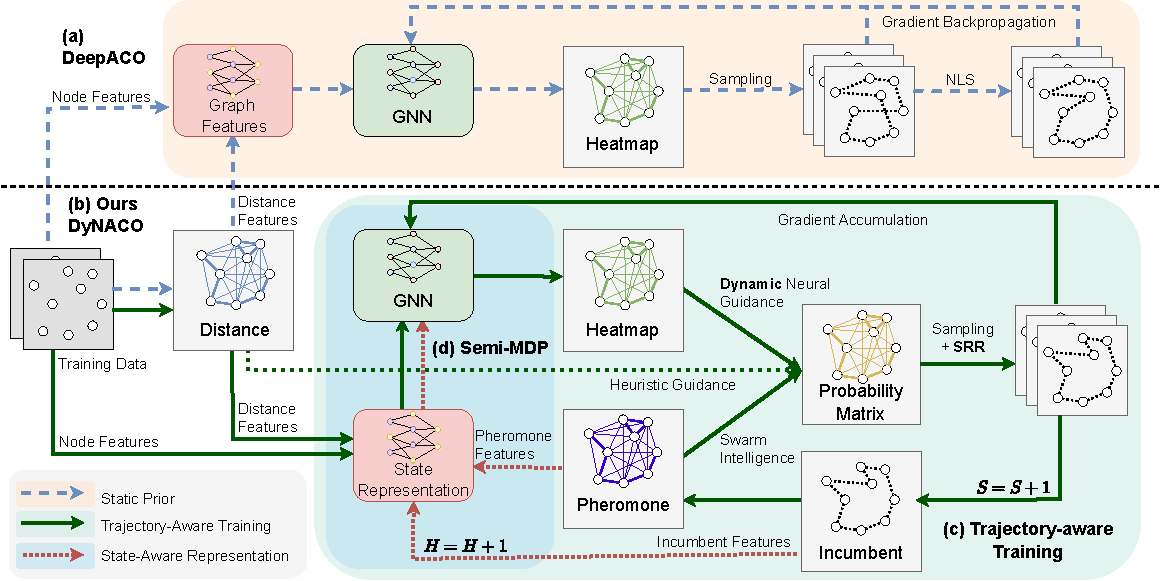
\includegraphics[width=\textwidth]{figures/overview.pdf}
\caption{\emph{Comparison of training paradigms and our \DyNACO{}.} (a) The original DeepACO paradigm~\cite{deepaco, gfacs, gtgaco}. (b) Our \DyNACO{} framework for dynamic guidance. (c) Trajectory-aware training that aligns with iterative search dynamics. (d) State-aware representation conditioning the policy on the evolving search state.}
\label{fig:guidance-loop}
\end{figure*}

% Standard ACO constructs solutions using transition probabilities $p(j \mid i) \propto [\tau_{ij}]^\alpha [\eta_{ij}]^\beta$, relying on an evolving pheromone matrix $\tau_{ij}$ but a strictly static heuristic visibility $\eta_{ij}$. 
% Based on the notation introduced in Section~\ref{sec:prelim}, we present \DyNACO{}, a dynamic neural-guided ACO framework that periodically observes the evolving search state and emits trajectory-aware edge guidance for the next block of ACO iterations.
% This section presents \DyNACO{}, 
Based on the notation introduced in Section~\ref{sec:prelim}, we present the method in the same progression used by the search system itself. We first define \DyNACO{}, Dynamic Neural Ant Colony Optimization: one state-aware policy repeatedly observes the evolving ACO state and emits guidance over the full search trajectory rather than committing to a one-shot heatmap. We then build \DyNACS{}, Dynamic Neural Ant Colony Search, on top of this base model by giving different ant groups complementary trajectory distributions within a shared colony. Finally, we describe the scalable search environment shared by both models: a perturbation-based ACO backend with scope-restricted refinement that makes the conceptual policy interface trainable and scalable. We instantiate the framework for Euclidean \TSP{} on $N$ nodes, seeking a tour $\pi$ that minimizes total cost $C(\pi)$, and for \CVRP{}, where we use a capacity-aware perturbation backend for feasibility handling.

\subsection{Semi-MDP Formulation}
\label{sec:mdp}
Prior neural-guided ACO methods~\cite{deepaco,gfacs,gtgaco} treat guidance as a \emph{one-shot prediction}: a network observes the instance graph and emits a static heatmap, trained from a single pheromone-free sample of ants, after which the solver runs a full ACO loop with pheromone dynamics to completion without further interaction. The model is therefore trained without pheromone dynamics. We address this mismatch by formalizing \DyNACO{} as a two-level hierarchy in which a neural \emph{meta-policy} $\pi_\theta$ repeatedly observes the macro-state and emits updated guidance, while the ACO backend executes $S$ iterations between observations. The policy follows the evolving ACO state rather than a fixed inference horizon, so it can be evaluated under longer ACO budgets by continuing to observe the current macro-state. Such a semi-MDP formulation enables:

\begin{enumerate}
\item \emph{Amortized policy updates.} The neural policy outputs actions only once every $S$ iterations and remains fixed during this interval. This amortizes overhead and effectively reduces variance during policy-gradient training.
\item \emph{Efficient PPO replay.} By framing the guidance process as a semi-MDP, we avoid tracking low-level internal ACO ant steps. To compute PPO importance ratios for off-policy reinforcement learning updates, we only need to store the macro-states at the update steps: the pheromone snapshots, incumbent features, and action traces.
\item \emph{Trajectory-aware objective.} Instead of a myopic single-step reward as used in the literature, we minimize the long-term cumulative cost $\sum_{h=1}^H C_h$ across the full MDP trajectory.
\end{enumerate}

Formally, we model this as a \emph{semi-MDP with fixed-duration macro-actions} as follows:
\begin{itemize}[topsep=0pt]
\item \emph{State} $\mathcal{S}_h = (G, \tau^{(h,0)}, b^{(h)})$: At update step $h$, the macro-state comprises the static $K$-nearest-neighbor candidate graph $G$, the pheromone matrix $\tau^{(h,0)} \in \mathbb{R}^{N \times K}$ at the start of the interval (indexed as $h,0$), and the current solution $b^{(h)}$.
\item \emph{Action} $a_h = z_\theta(\mathcal{S}_h) \in \mathbb{R}^{N \times K}$: A residual logit matrix emitted by the \DyNACO{} policy that shapes the pheromone matrix.
\item \emph{Transition} $P(\mathcal{S}_{h+1} \mid \mathcal{S}_h, a_h)$: The environment executes $S$ internal iterations of ACO (comprising ant sampling, scope-restricted refinement, and pheromone updates), functioning as a stochastic, state-dependent transition kernel.
\item \emph{Cost} $C_h = \frac{1}{S \cdot m} \sum_{s=1}^{S} \sum_{a=1}^{m} C(\hat{\pi}_{a,s})$: The average post-refinement tour cost across all $m$ ants over the $S$ iterations. Our objective is to minimize the expected cumulative cost $\sum_{h=1}^H C_h$.
\end{itemize}

% ======================================================================
% 3.3 State-Aware Policy and Training
% ======================================================================
\subsection{State-Aware Policy and Trajectory-Aware Training}
\label{sec:agent}


\smallskip\noindent\textbf{State-Aware Representation.}
\label{sec:state}
Prior neural-ACO methods condition solely on \emph{static} instance geometry, yielding guidance that cannot adapt to the solver's evolving state. The semi-MDP state $\mathcal{S}_h = (G,\, \tau^{(h,0)},\, b^{(h)})$ defined in Section~\ref{sec:mdp} isolates the two quantities that evolve between guidance updates: the pheromone field~$\tau$ and the incumbent solution~$b$. These are precisely the signals inherent to the ACO process; conditioning on them enables the semi-MDP formulation and renders the guidance \emph{dynamic}. We retain the static node features used by DeepACO~\cite{deepaco} for each problem and add three sparse edge channels on the $K$-NN graph: scale-normalized distance, local pheromone concentration, and an incumbent-edge indicator. The dynamic channels are recomputed at every outer step, remain bounded by $\mathcal{O}(N \cdot K)$, and are processed by a 12-layer GNN encoder~\cite{deepaco} with interleaved node and edge message passing. Appendix~\ref{app:features} gives the exact feature definitions.

The \DyNACO{} policy outputs a scalar guidance score $z_{ij}$ for each candidate edge via a 3-layer MLP decoder.
The shaped transition kernel adds these logits in log-space (Eq.~\ref{eq:held-logits}), corresponding to a KL-regularized policy where $p^\theta(\cdot\mid i) \propto q(j\mid i)\exp(z_{ij})$.
Because $\tau_{\min} > 0$ and logits remain finite, every candidate retains positive probability; the policy redistributes mass but cannot exclude edges.
\begin{algorithm}[t]
\caption{PPO training for dynamic \DyNACO{}.}
\label{alg:train}
\begin{algorithmic}[1]
\REQUIRE $\theta$ (policy params), $E$ (epochs), $H$ (outer steps), $S$ (inner steps), $K_{\text{PPO}}$ (PPO epochs), $m$ (ants)
\FOR{$e = 1 \to E$}
    \STATE $x \sim \mathcal{X}$; \, $\tau^{(1,0)} \gets \tau_{\max}$; \, $b^{(1)} \gets \textsc{Greedy}(x)$
    \FOR{$h = 1 \to H$}
        \STATE $z \gets z_{\theta_{\text{old}}}(\mathcal{S}_h)$; \, $\mathcal{D}_h \gets \emptyset$
            \COMMENT{Outer: emit guidance}
        \FOR{$s = 1 \to S$}
            \STATE $\{\pi_{a,s}\}_{a=1}^m \gets \textsc{Sample}(p^\theta, \tau^{(h,s)}, z, b^{(h)})$
                \COMMENT{Inner: ACO sampling}
            \STATE $\mathcal{D}_h \gets \mathcal{D}_h \cup \{(\tau^{(h,s)}, \{\pi_{a,s}\}, \{C(\hat{\pi}_{a,s})\})\}$
            \STATE $a^* \gets \argmin_a C(\hat{\pi}_{a,s})$; \, $b^{(h)} \gets \min(b^{(h)}, \hat{\pi}_{a^*,s})$
            \STATE $\tau^{(h,s+1)} \gets (1{-}\rho)\tau^{(h,s)} + \rho \cdot \Delta\tau(b^{(h)})$
        \ENDFOR
        \STATE $\tau^{(h+1,0)} \gets \tau^{(h,S)}$; \, $b^{(h+1)} \gets b^{(h)}$
        \FOR{$k = 1 \to K_{\text{PPO}}$}
            \STATE $\theta \gets \theta - \nabla_\theta \mathcal{L}^{\text{PPO}}(\theta; \mathcal{D}_h, z_\theta(\mathcal{S}_h))$
                \COMMENT{PPO update}
        \ENDFOR
    \ENDFOR
\ENDFOR
\end{algorithmic}
\end{algorithm}



\smallskip\noindent\textbf{Trajectory-Aware Training.}
\label{sec:training}
Prior methods~\cite{deepaco,gfacs,gtgaco} optimize a \emph{single-step} objective: $\min_\theta \mathbb{E}_{\pi \sim p_\theta(\cdot \mid G)} [ C(\pi) ]$, where ants sample once from the neural heuristic alone.
At inference, however, the same static heatmap is inserted into a full ACO loop where pheromone fields evolve over hundreds of iterations.
This discrepancy precludes learning adaptive behavior: because training never exposes the model to pheromone dynamics, the heatmap inevitably conflicts with the pheromone landscape in later iterations.

We instead optimize the expected per-iteration post-SRR cost across the full trajectory.
Let $\hat{\pi}_{a,s} = \mathrm{LS}(\pi_{a,s})$ denote the tour produced by ant $a$ at sampling iteration $s$ after local search:
\begin{equation}
J(\theta) = \mathbb{E} \left[ \frac{1}{I} \sum_{h=1}^H \sum_{s=1}^S \frac{1}{m} \sum_{a=1}^m C(\hat{\pi}_{a,s}) \right].
\end{equation}
This \emph{trajectory-aware} objective averages cost over all $I = H \times S$ iterations, training the policy to remain effective from early exploration through late exploitation and minimizing the area under the cost curve rather than a single endpoint.

Under perturbative sampling each ant modifies at most $M$ edges, and the log-probability of its trajectory is the sum over stochastic edge choices.
Because the number of stochastic decisions $T_a$ varies across ants (deterministic steps with a single feasible candidate contribute $\log p = 0$), we normalize by decision count: $\bar{\ell}_{a,s} = \frac{1}{T_a} \sum_{t=1}^{T_a} \log p^\theta(v_t \mid u_t)$.
This per-decision normalization prevents ants with more stochastic steps from dominating the gradient.
We compute a per-iteration baseline $b_s = \frac{1}{m}\sum_{a=1}^{m} C(\hat{\pi}_{a,s})$ and define advantage as $A_{a,s} = b_s - C(\hat{\pi}_{a,s})$, so that better-than-average tours receive positive advantage.
For PPO we normalize advantages across the batch: $\hat{A}_{a,s} = (A_{a,s} - \mu_A) / (\sigma_A + \epsilon)$.

% \begin{table*}[t]
% \centering
% \caption{Comparative results on synthetic \TSP{} and \CVRP{} instances. OOM: out of memory.}
% \label{tab:main-results}
% \small
% \renewcommand{\arraystretch}{0.8}
% \resizebox{\textwidth}{!}{
% \begin{tabular}{lcccccccccc}
% \toprule
% & \multicolumn{2}{c}{\TSP{}1K} & \multicolumn{2}{c}{\TSP{}5K} & \multicolumn{2}{c}{\TSP{}10K} & \multicolumn{2}{c}{\TSP{}50K} & \multicolumn{2}{c}{\TSP{}100K} \\
% \cmidrule(lr){2-3} \cmidrule(lr){4-5} \cmidrule(lr){6-7} \cmidrule(lr){8-9} \cmidrule(lr){10-11}
% Method & Obj.\ (Gap) & Time & Obj.\ (Gap) & Time & Obj.\ (Gap) & Time & Obj.\ (Gap) & Time & Obj.\ (Gap) & Time \\
% \midrule
% LKH3 & 23.12 (0.00\%) & 1.70m & 50.97 (0.00\%) & 12.00m & 71.78 (0.00\%) & 33.00m & 159.93 (0.00\%) & 10.00h & 225.99 (0.00\%) & 25.00h \\
% \midrule
% H-TSP & 24.66 (6.66\%) & 48.00s & 55.16 (8.22\%) & 1.20m & 77.75 (8.32\%) & 2.20m & OOM & OOM & OOM & OOM \\
% GLOP & 23.78 (2.85\%) & 10.20s & 53.15 (4.28\%) & 1.00m & 75.04 (4.54\%) & 1.90m & 168.09 (5.10\%) & 1.50m & 237.61 (5.14\%) & 3.90m \\
% INViT-3V greedy & 24.66 (6.66\%) & 9.00s & 54.49 (6.91\%) & 1.20m & 76.85 (7.06\%) & 3.70m & 171.42 (7.18\%) & 1.30h & 242.26 (7.20\%) & 5.00h \\
% L2C-Insert greedy & 24.22 (4.75\%) & 0.16s & -- & - & 77.34 (7.75\%) & 3.98s & 171.78 (7.41\%) & 19.80s & 242.76 (7.42\%) & 39.49s \\
% SIL greedy & 23.57 (1.94\%) & 0.20s & 52.59 (3.18\%) & 5.20s & 74.69 (4.05\%) & 20.10s & 168.50 (5.36\%) & 7.70m & 239.84 (6.13\%) & 33.00m \\
% POMO aug×8 & 32.51 (40.61\%) & 4.10s & 87.72 (72.10\%) & 8.60m & OOM & OOM & OOM & OOM & OOM & OOM \\
% BQ bs16 & 23.43 (1.34\%) & 13.00s & 58.27 (14.32\%) & 24.00s & OOM & OOM & OOM & OOM & OOM & OOM \\
% SIGD bs16 & 23.36 (1.04\%) & 17.30s & 55.77 (9.42\%) & 30.50m & OOM & OOM & OOM & OOM & OOM & OOM \\
% LEHD RRC$_{1000}$ & 23.29 (0.74\%) & 3.30m & 54.43 (6.79\%) & 8.60m & 80.90 (12.71\%) & 18.60m & OOM & OOM & OOM & OOM \\
% L2C-Insert (I$_{1000}$) & 23.23 (0.48\%) & 21.75s & -- & - & 73.27 (2.08\%) & 1.04m & 166.06 (3.83\%) & 1.30m & 237.11 (4.92\%) & 1.63m \\
% SIL PRC$_{10}$ & 23.40 (1.19\%) & 0.90s & 52.36 (2.73\%) & 5.10s & 73.99 (3.08\%) & 10.00s & 166.69 (4.23\%) & 1.33m & 235.38 (4.16\%) & 3.00m \\
% SIL PRC$_{1000}$ & 23.21 (0.38\%) & 1.50m & 51.67 (1.37\%) & 9.40m & 73.08 (1.81\%) & 17.00m & 163.95 (2.51\%) & 1.38h & 231.52 (2.45\%) & 2.60h \\
% \midrule
% ACO I$_{1000}$ & 23.31 (0.83\%) & 0.54s & 52.12 (2.26\%) & 1.54s & 73.80 (2.82\%) & 2.66s & 168.17 (5.15\%) & 11.86s & 241.26 (6.76\%) & 25.02s \\
% ACO I$_{2000}$ & 23.28 (0.70\%) & 1.08s & 51.98 (1.98\%) & 3.11s & 73.54 (2.46\%) & 5.30s & 166.25 (3.95\%) & 23.07s & 237.53 (5.10\%) & 47.56s \\
% ACO I$_{5000}$ & 23.25 (0.55\%) & 2.72s & 51.88 (1.78\%) & 7.74s & 73.33 (2.15\%) & 13.41s & 164.90 (3.11\%) & 56.43s & 234.33 (3.69\%) & 1.89m \\
% ACO I$_{10000}$ & 23.23 (0.48\%) & 5.44s & 51.81 (1.65\%) & 15.59s & 73.23 (2.02\%) & 26.81s & 164.38 (2.78\%) & 1.87m & 233.04 (3.12\%) & 3.72m \\
% \midrule
% DyNACO I$_{1000}$ & 23.24 (0.52\%) & 0.37s & 51.63 (1.30\%) & 1.19s & 72.92 (1.59\%) & 1.94s & 167.36 (4.64\%) & 9.50s & 241.20 (6.73\%) & 21.52s \\
% DyNACO I$_{2000}$ & 23.21 (0.39\%) & 0.73s & 51.52 (1.08\%) & 2.23s & 72.67 (1.24\%) & 3.72s & 164.58 (2.91\%) & 17.31s & 236.68 (4.73\%) & 38.45s \\
% DyNACO I$_{5000}$ & 23.18 (0.27\%) & 1.85s & 51.41 (0.86\%) & 5.30s & 72.48 (0.97\%) & 9.06s & 162.66 (1.71\%) & 40.64s & 232.07 (2.69\%) & 1.48m \\
% DyNACO I$_{10000}$ & \textbf{23.17} (\textbf{0.20\%}) & 3.68s & \textbf{51.35} (\textbf{0.75\%}) & 10.42s & \textbf{72.37} (\textbf{0.82\%}) & 17.89s & \textbf{161.93} (\textbf{1.25\%}) & 1.33m & \textbf{230.28} (\textbf{1.90\%}) & 2.86m \\
% \midrule
% \midrule
% & \multicolumn{2}{c}{\CVRP{}1K} & \multicolumn{2}{c}{\CVRP{}5K} & \multicolumn{2}{c}{\CVRP{}10K} & \multicolumn{2}{c}{\CVRP{}50K} & \multicolumn{2}{c}{\CVRP{}100K} \\
% \cmidrule(lr){2-3} \cmidrule(lr){4-5} \cmidrule(lr){6-7} \cmidrule(lr){8-9} \cmidrule(lr){10-11}
% Method & Obj.\ (Gap) & Time & Obj.\ (Gap) & Time & Obj.\ (Gap) & Time & Obj.\ (Gap) & Time & Obj.\ (Gap) & Time \\
% \midrule
% HGS & 36.29 (0.00\%) & 2.50m & 89.74 (0.00\%) & 2.00h & 107.40 (0.00\%) & 5.00h & 267.73 (0.00\%) & 8.10h & 476.11 (0.00\%) & 24.00h \\
% GLOP-G (LKH3) & 39.50 (8.85\%) & 1.30s & 98.90 (10.21\%) & 6.80s & 116.28 (8.27\%) & 11.20s & OOM & OOM & OOM & OOM \\
% \midrule
% POMO aug×8 & 84.89 (133.92\%) & 4.80s & 393.27 (338.23\%) & 11.00m & OOM & OOM & OOM & OOM & OOM & OOM \\
% LEHD RRC$_{1000}$ & 37.43 (3.14\%) & 3.40m & 101.07 (12.63\%) & 31.00m & 138.73 (29.17\%) & 41.00m & OOM & OOM & OOM & OOM \\
% BQ bs16 & 38.17 (5.18\%) & 14.00s & 104.40 (16.34\%) & 2.60m & OOM & OOM & OOM & OOM & OOM & OOM \\
% SIGD bs16 & 39.15 (7.88\%) & 17.30s & 103.46 (15.29\%) & 1.91m & 131.48 (22.42\%) & 3.97m & 477.43 (78.33\%) & 25.90m & OOM & OOM \\
% INViT-3V greedy & 42.75 (17.80\%) & 11.40s & 109.85 (22.41\%) & 1.40m & 141.41 (31.67\%) & 4.20m & 402.05 (50.17\%) & 2.90h & 688.80 (44.67\%) & 8.30h \\
% LEHD greedy & 38.91 (7.22\%) & 0.80s & 105.61 (17.68\%) & 1.56m & 146.24 (36.16\%) & 11.85m & OOM & OOM & OOM & OOM \\
% L2C-Insert greedy & 39.69 (9.36\%) & 0.41s & 109.45 (21.96\%) & 3.30s & 147.98 (37.78\%) & 6.64s & 419.51 (56.69\%) & 33.83s & 722.17 (51.68\%) & 1.14m \\
% L2C-Insert I$_{1000}$ & 38.33 (5.63\%) & 43.59s & 103.60 (15.45\%) & 1.21m & 135.77 (26.42\%) & 1.27m & 389.86 (45.62\%) & 1.74m & 692.95 (45.54\%) & 2.38m \\
% SIL PRC$_{10}$ & 37.93 (4.52\%) & 0.70s & 93.92 (4.66\%) & 3.90s & 112.17 (4.44\%) & 6.80s & 285.20 (6.53\%) & 28.00s & 496.24 (4.23\%) & 59.00s \\
% SIL PRC$_{1000}$ & 37.28 (2.73\%) & 1.50m & \textbf{90.81} (\textbf{1.19\%}) & 8.80m & \textbf{106.69} (\textbf{-0.66\%}) & 15.20m & \textbf{262.82} (\textbf{-1.83\%}) & 1.04h & \textbf{463.95} (\textbf{-2.55\%}) & 2.17h \\
% \midrule
% ACO I$_{1000}$ & 37.48 (3.28\%) & 2.03s & 97.00 (8.09\%) & 4.21s & 119.78 (11.53\%) & 7.32s & 303.58 (13.39\%) & 31.73s & 528.31 (10.96\%) & 1.15m \\
% ACO I$_{2000}$ & 37.27 (2.71\%) & 4.04s & 95.88 (6.84\%) & 8.43s & 118.24 (10.10\%) & 14.71s & 299.46 (11.85\%) & 1.06m & 523.14 (9.88\%) & 2.30m \\
% ACO I$_{5000}$ & 37.09 (2.20\%) & 10.09s & 94.73 (5.57\%) & 21.10s & 116.07 (8.08\%) & 35.87s & 294.24 (9.90\%) & 2.68m & 516.05 (8.39\%) & 5.77m \\
% ACO I$_{10000}$ & 36.96 (1.85\%) & 20.17s & 93.76 (4.48\%) & 42.26s & 114.66 (6.76\%) & 1.24m & 290.70 (8.58\%) & 5.38m & 510.70 (7.26\%) & 11.55m \\
% \midrule
% DyNACO I$_{1000}$ & 37.30 (2.79\%) & 1.79s & 95.92 (6.89\%) & 4.28s & 119.26 (11.04\%) & 7.93s & 302.10 (12.84\%) & 34.73s & 525.91 (10.46\%) & 1.18m \\
% DyNACO I$_{2000}$ & 37.11 (2.26\%) & 3.56s & 94.92 (5.78\%) & 8.46s & 117.90 (9.78\%) & 15.87s & 299.17 (11.74\%) & 1.16m & 521.58 (9.55\%) & 2.37m \\
% DyNACO I$_{5000}$ & 36.80 (1.42\%) & 9.58s & 93.70 (4.41\%) & 21.37s & 115.37 (7.42\%) & 38.30s & 293.35 (9.57\%) & 2.84m & 513.55 (7.86\%) & 5.86m \\
% DyNACO I$_{10000}$ & \textbf{36.67} (\textbf{1.04\%}) & 19.05s & 92.75 (3.36\%) & 42.87s & 113.89 (6.04\%) & 1.28m & 289.87 (8.27\%) & 5.60m & 508.23 (6.75\%) & 11.70m \\
% \bottomrule
% \end{tabular}
% }
% \end{table*}

% \include{tables/table1}

We optimize using PPO with trajectory replay.
After collecting trajectories for $S$ sampling iterations under $\pi_{\theta_{\text{old}}}$, we perform $K_{\text{PPO}}$ optimization epochs using the clipped surrogate:
\begin{multline}
\mathcal{L}^{\mathrm{PPO}}(\theta)
= -\mathbb{E}_{a,s}\Big[\min\big(
 r_{a,s}(\theta)\hat{A}_{a,s},\\
\operatorname{clip}\!\left(r_{a,s}(\theta),1-\epsilon,1+\epsilon\right)
\hat{A}_{a,s}\big)\Big].
\end{multline}
where $r_{a,s}(\theta) = \pi_\theta(\pi_{a,s} | \mathcal{S}_h) / \pi_{\theta_{\text{old}}}(\pi_{a,s} | \mathcal{S}_h)$, $\epsilon=0.1$, and $\hat{A}_{a,s}$ is the normalized advantage.
The semi-MDP interface makes this replay memory-efficient. For each outer step, we store the incumbent successor array needed to reconstruct incumbent-derived edge features. For each inner iteration, we store the sparse pheromone snapshot, the stochastic action trace of each ant, the feasible-candidate mask at each stochastic decision, and the post-refinement costs. These quantities are sufficient to recompute PPO log-probabilities under the current policy because the transition probability depends only on the shaped kernel and the stored feasible set; deterministic steps with a single feasible candidate contribute zero log-probability. Thus, \DyNACO{} can recompute importance ratios without storing the full GNN computation graph, while all state features remain on the sparse $K$-NN graph with $\mathcal{O}(nK)$ memory.
The full procedure for the dynamic base model is given in Algorithm~\ref{alg:train}. \DyNACO{} resolves the static-heatmap limitation by making guidance state-aware and trajectory-trained. However, it still applies one behavior to the whole ant population. The next section addresses this remaining limitation by extending the single-behavior policy into trajectory-diverse guidance.


\section{Trajectory-Diverse Neural Ant Colony Search}
\label{sec:multi-trajectory}
The previous section defines \DyNACO{} as the dynamic base model: one state-aware policy observes the evolving ACO macro-state and emits one guidance field for the next search interval. This resolves the static-heatmap limitation, but it still leaves the colony with only one learned behavior. ACO is a population-based optimizer, and its strength comes partly from maintaining several compatible ways of exploring the same search state. A single neural guidance field imposes one ordering of candidate perturbations on the whole ant population, which can be restrictive when pheromone has concentrated or when an out-of-distribution instance admits several plausible continuation modes.

Motivated by recent NCO work on learned strategy diversity~\cite{mdam,poppy,polynet}, we introduce \DyNACS{}, which builds on \DyNACO{} by learning a mixture of trajectory distributions. Each behavior guides a subset of ants, while all ants still interact through the same incumbent solution and pheromone field. This design forms a closed-loop trajectory-diverse search process. First, the policy maps the current ACO state to complementary edge-level guidance. Second, these behaviors generate heterogeneous perturbation trajectories that are evaluated under the same refinement operator. Third, successful perturbations are written back to shared search memory and influence the distributions used in later steps. Finally, online behavior routing assigns search effort according to recent refined-solution quality, adapting the mixture to the current instance without gradient updates.

\begin{figure}[t]
    \centering

    \subfloat[Single guidance field]{%
        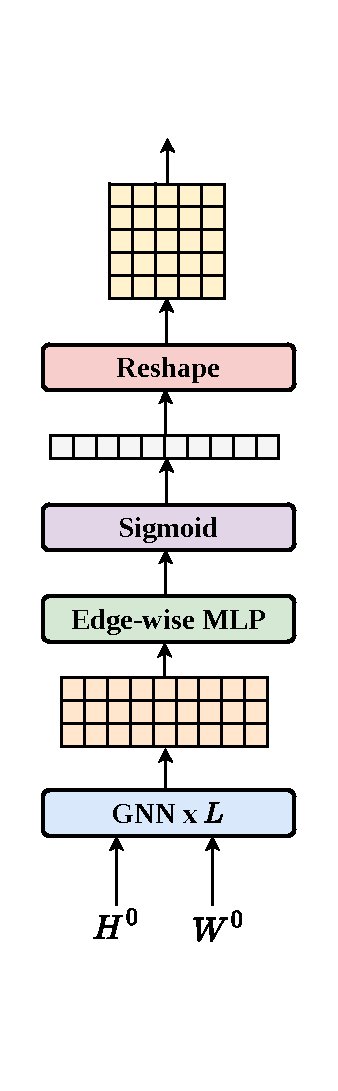
\includegraphics[height=0.34\textheight]{figures/gnn.pdf}%
    }
    \subfloat[Multi-trajectory guidance]{%
        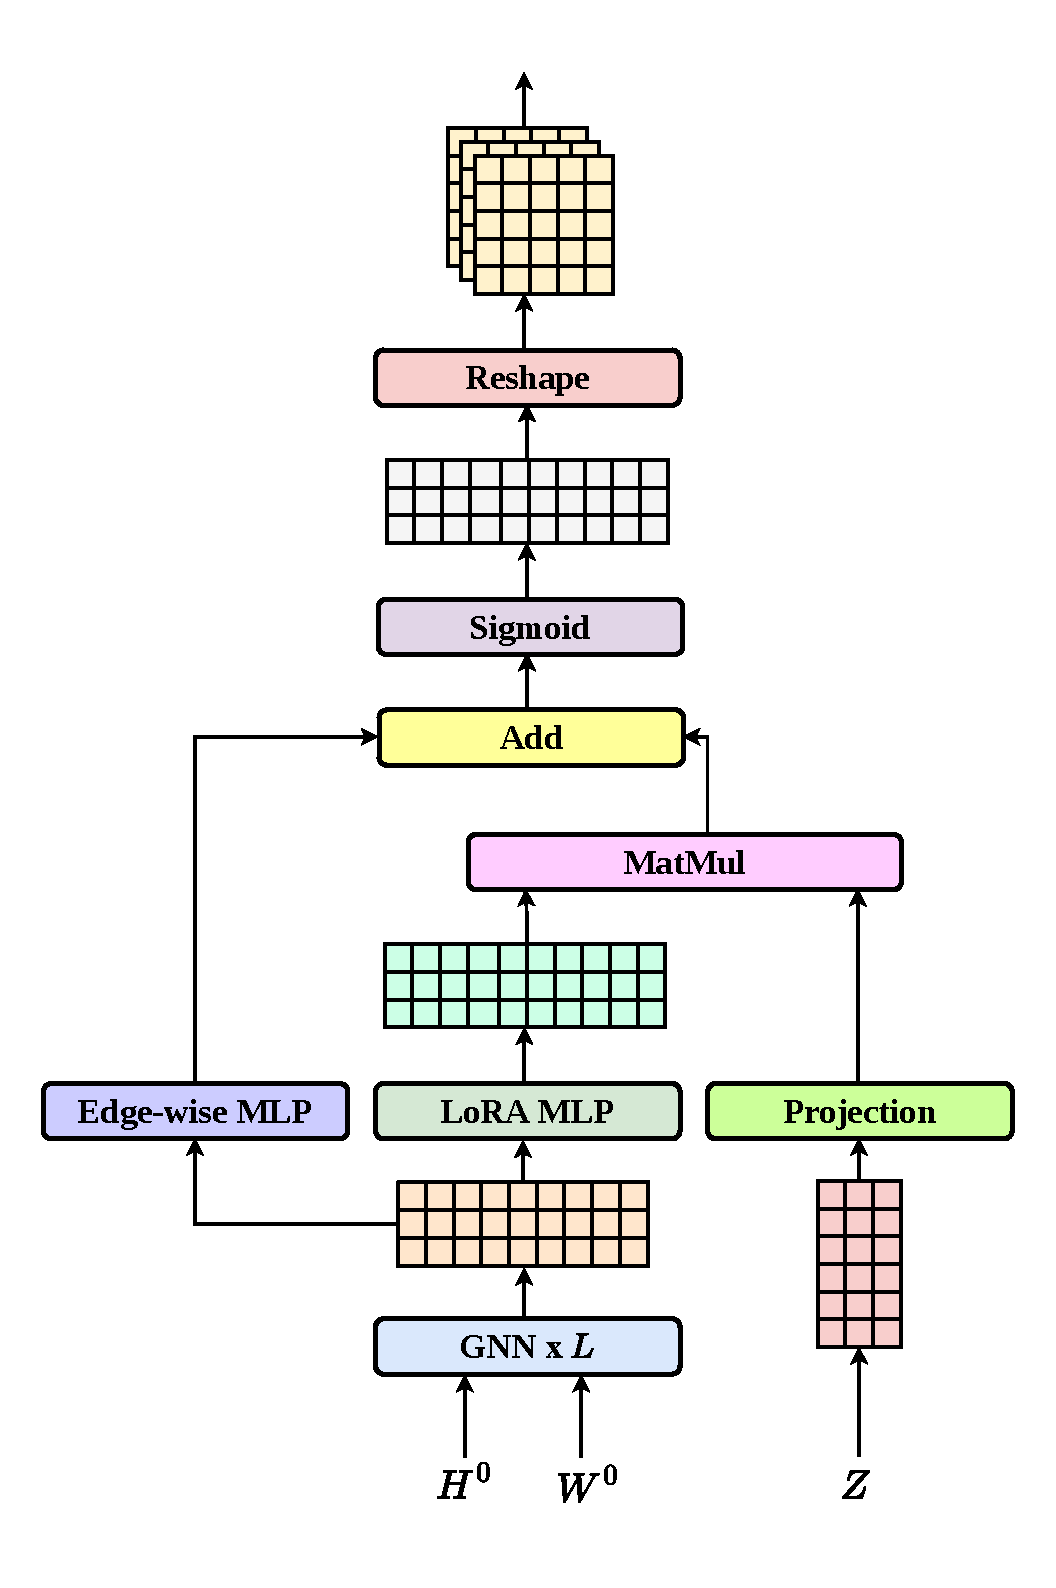
\includegraphics[height=0.34\textheight]{figures/moe.pdf}%
    }\hfill

\caption{Comparison between a single dynamic guidance field and trajectory-diverse guidance. The \DyNACO{} policy maps each macro-state to one sparse guidance field, whereas \DyNACS{} maps the same state to multiple guidance fields that steer disjoint ant groups within one shared search process.}
    \label{fig:multi-head-lora-gnn}
\end{figure}

\subsection{Mixture-Based Trajectory Guidance}
\label{sec:tdg-formulation}

We extend the semi-MDP in Section~\ref{sec:mdp} by augmenting dynamic guidance with a discrete behavior index. At macro-step $h$, the state remains
\begin{equation}
\mathcal{S}_h=(G,\tau^{(h,0)},b^{(h)}),
\end{equation}
but the policy action is now a set of $R$ behavior-conditioned guidance fields,
\begin{equation}
a_h = \{z_\theta^{(r)}(\mathcal{S}_h)\}_{r=1}^{R},
\qquad
z_\theta^{(r)}(\mathcal{S}_h)\in\mathbb{R}^{N\times K}.
\end{equation}
Each behavior $r$ defines a trajectory distribution for ants assigned to that behavior:
\begin{equation}
\log p_r^\theta(j \mid i; h, s)
= \alpha \log \tau^{(h,s)}_{ij}
+ \beta \log \eta_{ij}
+ \gamma z_{ij}^{(r)}(\mathcal{S}_h).
\label{eq:multi-trajectory-kernel}
\end{equation}
Thus, \DyNACS{} does not run $R$ independent solvers. It defines $R$ behavior-conditioned distributions over perturbation trajectories while preserving the same macro-state, incumbent solution, pheromone update, and SRR projection.

Let $\mathcal{A}_r^{(h,s)}$ be the ants assigned to behavior $r$ at inner iteration $s$. The transition cost for a macro-step is still measured over the combined population,
\begin{equation}
C_h =
\frac{1}{S m}\sum_{s=1}^{S}\sum_{r=1}^{R}
\sum_{a\in\mathcal{A}_r^{(h,s)}} C(\hat{\pi}_{a,s}),
\end{equation}
but each trajectory log-probability is evaluated under its assigned behavior,
\begin{equation}
\log \pi_\theta(\pi_{a,s}, r\mid\mathcal{S}_h)
= \log \omega_r^{(h)}
+ \sum_{t=1}^{T_a}\log p_r^\theta(v_t\mid u_t;h,s),
\end{equation}
where $\omega_r^{(h)}$ is the routing weight for behavior $r$. This formulation turns neural guidance from one homogeneous transition bias into a mixture of trajectory distributions: each behavior is evaluated through the quality of its refined trajectories, while all behaviors cooperate through the shared colony state.

\subsection{Behavior-Conditioned Guidance Generation}
\label{sec:tdg-policy}

The mixture model shares the state representation used by \DyNACO{} and learns multiple behavior-conditioned guidance maps on top of that representation. Let
\begin{equation}
\{e_{ij}^{(h)}\}_{(i,j)\in G}
=
\operatorname{GNN}_{\theta}
\bigl(G,\tau^{(h,0)},b^{(h)}\bigr)
\end{equation}
denote the sparse edge embeddings produced from the current macro-state. A shared guidance map $g_0$ captures common preferences over candidate edges, while $R$ behavior-conditioned residual maps $\{\Delta_r\}_{r=1}^{R}$ specialize this representation into distinct trajectory biases:
\begin{equation}
z_{ij}^{(r)}(\mathcal{S}_h)
= g_0(e_{ij}^{(h)}) + \Delta_r(e_{ij}^{(h)}),
\qquad r=1,\ldots,R,
\label{eq:multi-trajectory-logit}
\end{equation}
This parameterization makes the behavior-conditioned distributions comparable because they are grounded in the same encoded search state, while the residual maps let them express different edge-ordering preferences. In this sense, the mixture is not a collection of independent policies; it is a structured factorization of one state-aware policy into a shared search representation and multiple behavior-conditioned guidance maps.

We use a low-rank parameterization for the residual behavior maps to keep the mixture lightweight. In one equivalent form, the behavior-specific map is
\begin{equation}
W_r = W_0 + \frac{\alpha_{\mathrm{L}}}{d_{\mathrm{L}}}B_rA_r,
\end{equation}
where $W_0$ is shared, $A_r$ and $B_r$ are behavior-specific low-rank factors, and $d_{\mathrm{L}}$ is the adapter rank. Equivalently, the residual map can be written as
\begin{equation}
\Delta_r(e_{ij}^{(h)})
= \phi(e_{ij}^{(h)})^\top \psi_r + c_r,
\end{equation}
with an edge factor $\phi(\cdot)$ and a behavior code $\psi_r$. Both forms preserve the main computational property: the GNN is evaluated once per macro-state, and the mixture adds only lightweight behavior-specific maps. The resulting output is a sparse tensor in $\mathbb{R}^{R\times N\times K}$, matching the candidate graph used by the ACO backend.

\subsection{Shared Search Memory}
\label{sec:tdg-shared-colony}

At each inner ACO iteration, the ant population is partitioned into groups $\{\mathcal{A}_r\}_{r=1}^R$. Ants in group $r$ sample perturbation trajectories under $p_r^\theta$, but all groups start from the same reference solution and contribute to the same post-SRR candidate pool. The best refined trajectory among the combined population updates the incumbent, and the shared pheromone field is updated from that incumbent. The next macro-state therefore aggregates the effect of all behavior-conditioned distributions:
\begin{equation}
\mathcal{S}_{h+1}
=
\mathcal{T}_{\mathrm{ACO}}
\bigl(\mathcal{S}_h,\{z_\theta^{(r)}(\mathcal{S}_h)\}_{r=1}^{R}\bigr).
\end{equation}
This coupling is the key difference between trajectory-diverse guidance and independent multi-start search. Independent colonies would maintain separate pheromone fields and exchange information only through final solution selection. In \DyNACS{}, the behaviors interact through shared search memory at every inner iteration: a behavior that discovers a useful perturbation can reinforce the common colony state, while other behaviors can later exploit or counteract that reinforcement.

\subsection{Online Behavior Routing}
\label{sec:tdg-allocation}

The simplest trajectory-diverse variant routes ants uniformly across behaviors. We also use an online routing rule that shifts ant budget toward behaviors that have recently produced stronger refined trajectories. The rule keeps inference lightweight: it updates only running utilities and integer ant counts, without changing network parameters or maintaining separate solver states. Let $u_r^{(h)}$ denote the running utility for behavior $r$ at macro-step $h$, where larger values indicate better recent performance. Given the refined costs from ants assigned to behavior $r$, we form a per-step score
\begin{equation}
s_r^{(h)}
= -\operatorname{TopQMean}_{a\in\mathcal{A}_r}
\!\left[C(\hat{\pi}_{a,h})\right],
\label{eq:trajectory-prior-score}
\end{equation}
where the top-$Q$ mean reduces sensitivity to a single lucky ant and becomes the negative best cost when $Q=1$. Scores are normalized across behaviors and accumulated with an exponential moving average,
\begin{equation}
u_r^{(h+1)}
= (1-\mu)u_r^{(h)}+\mu\,\operatorname{Norm}(s_r^{(h)}).
\end{equation}
The next routing weights are
\begin{equation}
w_r^{(h+1)}
=
\frac{\exp(u_r^{(h+1)}/\lambda)}
{\sum_{r'=1}^{R}\exp(u_{r'}^{(h+1)}/\lambda)}.
\label{eq:trajectory-prior-weights}
\end{equation}
We then project $m w_r^{(h+1)}$ to integer ant counts $m_r^{(h+1)}$ with $\sum_r m_r^{(h+1)}=m$ and at least one ant for each active behavior. Uniform routing is recovered by fixing $w_r=1/R$. The rule changes only which behavior each ant follows; it does not create separate pheromone states or separate local-search procedures.

\subsection{Training and Inference}
\label{sec:tdg-training}

Training \DyNACS{} uses the same trajectory-aware PPO interface as \DyNACO{}, but conditions the trajectory likelihood on the assigned behavior. During training, the mixture acts as a strategy-discovery mechanism: all behaviors are evaluated through the shared colony, and the policy update is formed from the strongest behavior-conditioned trajectory group in that rollout. During inference, the learned behavior-conditioned maps are fixed and only the routing weights change online, allowing the search to adapt to the current instance without gradient updates. Let
\begin{equation}
r_h^\star = \operatorname*{arg\,max}_{r\in\{1,\ldots,R\}} s_r^{(h)}
\end{equation}
denote the behavior with the best refined trajectory score at macro-step $h$. For an ant assigned to this behavior, the PPO ratio is
\begin{equation}
\rho_{a,s}^{(r_h^\star)}(\theta)
=
\exp\!\left(
\bar{\ell}_{a,s}^{(r_h^\star)}(\theta)
-\bar{\ell}_{a,s}^{(r_h^\star)}(\theta_{\mathrm{old}})
\right),
\end{equation}
where $\bar{\ell}_{a,s}^{(r_h^\star)}$ is the per-decision normalized log-probability under $p_{r_h^\star}^\theta$. The clipped objective is applied to the selected behavior-conditioned trajectories:
\begin{multline}
\mathcal{L}_{\mathrm{TD}}(\theta)
= -\mathbb{E}_{a\in\mathcal{A}_{r_h^\star},s}\Big[
\min\big(
\rho_{a,s}^{(r_h^\star)}(\theta)\hat{A}_{a,s},\\
\operatorname{clip}(\rho_{a,s}^{(r_h^\star)}(\theta),1-\epsilon,1+\epsilon)
\hat{A}_{a,s}\big)\Big].
\end{multline}
The other behaviors are still part of the search transition because their refined trajectories can update the shared incumbent, pheromone field, and future routing utilities. Optionally, a small information-theoretic diversity regularizer can be applied to the mixture by maximizing the Jensen divergence among the row-wise transition distributions induced by $\{z^{(r)}\}_{r=1}^R$. This regularizer is not a separate solver objective; it only discourages all behaviors from collapsing to the same transition distribution.

\begin{algorithm}[t]
\caption{Trajectory-diverse guidance with online behavior routing for \DyNACS{}.}
\label{alg:trajectory-diverse}
\begin{algorithmic}[1]
\REQUIRE $\theta$ (shared encoder and behavior-conditioned maps), $R$ (behaviors), $m$ (ants), $H$ (outer steps), $S$ (inner steps)
\STATE Initialize $\tau^{(1,0)} \gets \tau_{\max}$, $b^{(1)} \gets \textsc{Greedy}(x)$, and routing utilities $\{u_r^{(1)}\}_{r=1}^R$
\FOR{$h = 1 \to H$}
    \STATE Encode $\mathcal{S}_h=(G,\tau^{(h,0)},b^{(h)})$
    \STATE Emit behavior-conditioned guidance fields $\{z_\theta^{(r)}(\mathcal{S}_h)\}_{r=1}^R$
    \STATE Route ants $\{m_r^{(h)}\}_{r=1}^R$ using uniform weights or Eqs.~\eqref{eq:trajectory-prior-score}--\eqref{eq:trajectory-prior-weights}
    \FOR{$s = 1 \to S$}
        \FOR{$r = 1 \to R$}
            \STATE Sample $m_r^{(h)}$ perturbation trajectories under $p_r^\theta(\cdot \mid \mathcal{S}_h,\tau^{(h,s)})$
        \ENDFOR
        \STATE Apply SRR to all sampled trajectories
        \STATE Update $b^{(h)}$ with the best refined trajectory from the combined population
        \STATE Update $\tau^{(h,s+1)}$ using the shared incumbent
        \STATE Update routing utilities $\{u_r\}_{r=1}^R$ from refined trajectory costs
    \ENDFOR
    \STATE $\tau^{(h+1,0)} \gets \tau^{(h,S)}$; \, $b^{(h+1)} \gets b^{(h)}$
\ENDFOR
\end{algorithmic}
\end{algorithm}


% ======================================================================
% 3.2 The Perturbative Environment
% ======================================================================
\section{Scalable Search Environment}
\label{sec:computational-alignment}
\label{sec:backend}

The previous two sections define what the policy observes and how one or several guidance fields shape search behavior. We now give the search environment through which those policy outputs affect the solver. This environment is shared by \DyNACO{} and \DyNACS{}: it converts edge-level guidance into short stochastic perturbation trajectories, then projects those trajectories back to locally consistent solutions before rewards are assigned. Its role is to keep the neural decision horizon short enough for policy learning while preserving the refinement quality expected from ACO\@. We realize this environment with two mechanisms: \emph{perturbative sampling}, which changes the action object from a full tour to a small set of edge interventions, and \emph{Scope-Restricted Refinement (SRR)}, which performs local projection around the affected region so that rewards remain causally tied to the sampled interventions.

\smallskip\noindent\textbf{Perturbative Sampling.}
In prior neural-guided ACO frameworks~\cite{deepaco,gfacs,gtgaco}, each ant constructs a tour from scratch. This makes the policy responsible for a sequence of $N$ edge decisions, which becomes expensive at large scales and exposes learning to sequential error accumulation. It also leaves no explicit reference state around which a post-processing step can preserve credit assignment. We instead use the current incumbent as a reference trajectory and let each ant modify only a small subset of candidate edges on a sparse $K$-nearest-neighbor graph. For \TSP{}, this perturbation interface follows~\cite{faco}; for \CVRP{}, we instantiate the same interface with capacity-aware feasibility checks (Appendix~\ref{app:backend}).

At sampling iteration $s$ of guidance update $h$, transition probabilities combine pheromones, heuristics, and neural guidance via a \emph{guidance weight} $\gamma$:
\begin{equation}
\log p^\theta(j \mid i; h, s) = \alpha \log \tau^{(h,s)}_{ij} + \beta \log \eta_{ij} + \gamma\, z_{ij}(\mathcal{S}_h).
\label{eq:held-logits}
\end{equation}
During training $\gamma{=}1$ (constant forcing); at inference $\gamma$ may be annealed (see Section~\ref{sec:inference}). The policy outputs $z_\theta(\mathcal{S}_h)$ once per guidance update and holds it constant for $S$ sampling iterations, decoupling neural guidance (updated at guidance-update boundaries) from pheromone dynamics (updated at every sampling iteration). Crucially, prior neural-ACO methods~\cite{deepaco,gfacs,gtgaco} replace the heuristic term~$\eta_{ij}$ with neural output, discarding hand-crafted domain knowledge. We instead retain both $\tau_{ij}$ and $\eta_{ij}$, and introduce neural logits~$z_{ij}$ as a third, additive term in Eq.~\eqref{eq:held-logits}. This preserves the domain knowledge encoded in $\eta$ while letting the network provide complementary, state-dependent guidance.

Formally, each ant initializes from the incumbent solution $b^{(h)}$ and executes up to $M$ stochastic edge interventions. At each intervention, the ant samples a successor node $v$ from the feasible candidate set according to Eq.~\eqref{eq:held-logits}; edges $(u,v)$ absent from the incumbent are recorded as anchors for the subsequent scope-restricted refinement mechanism. The trajectory log-probability decomposes over stochastic decisions:
\begin{equation}
\log \pi_\theta(\pi_{a,s} \mid \mathcal{S}_h) = \sum_{t=1}^{T_a} \log p^\theta(v_t \mid u_t; h, s),
\label{eq:logp-trajectory}
\end{equation}
where $T_a \le M$ denotes the number of stochastic interventions, i.e., steps at which multiple candidates were feasible. This formulation changes the learning problem from constructing all $N$ tour edges to selecting a small intervention set of size at most $M \ll N$. Consequently, the decision horizon is bounded by $M$ rather than $N$, preventing the error accumulation inherent in $\mathcal{O}(N)$-length sequential construction and stabilizing policy learning at scale. The localized intervention set also defines the region on which refinement should be allowed to affect the reward.

\smallskip\noindent\textbf{Scope-Restricted Refinement.}
\label{sec:localized-ls}
In neural-guided ACO~\cite{deepaco,gfacs,gtgaco}, refinement is part of the training environment: the post-refinement cost is the reward signal used for policy-gradient updates. This creates a projection-credit trade-off. If refinement is too weak, sampled trajectories remain under-refined and rewards are noisy. If refinement is too strong and unconstrained, it can rewrite most of the sampled intervention, so the final cost reflects the refinement heuristic rather than the neural decision. We refer to this failure mode as \emph{gradient washout}.

Figure~\ref{fig:credit_assignment} illustrates this trade-off using DeepACO on TSP-200 under three refinement strategies. With \emph{Full 2-opt} (red), the policy fails to converge because the local search heavily rewrites the sampled tour and severs the causal link between actions and rewards. \emph{Limited 2-opt} (orange) preserves more of the learning signal by stopping after $N/4$ swaps, but this early stopping bottlenecks solution quality. \emph{Neural Local Search}~\cite{deepaco} (blue) improves quality by using the neural policy to score candidate swaps, but it is not scalable because it requires neural evaluations inside the refinement loop.

\begin{figure}[t]
    \centering
    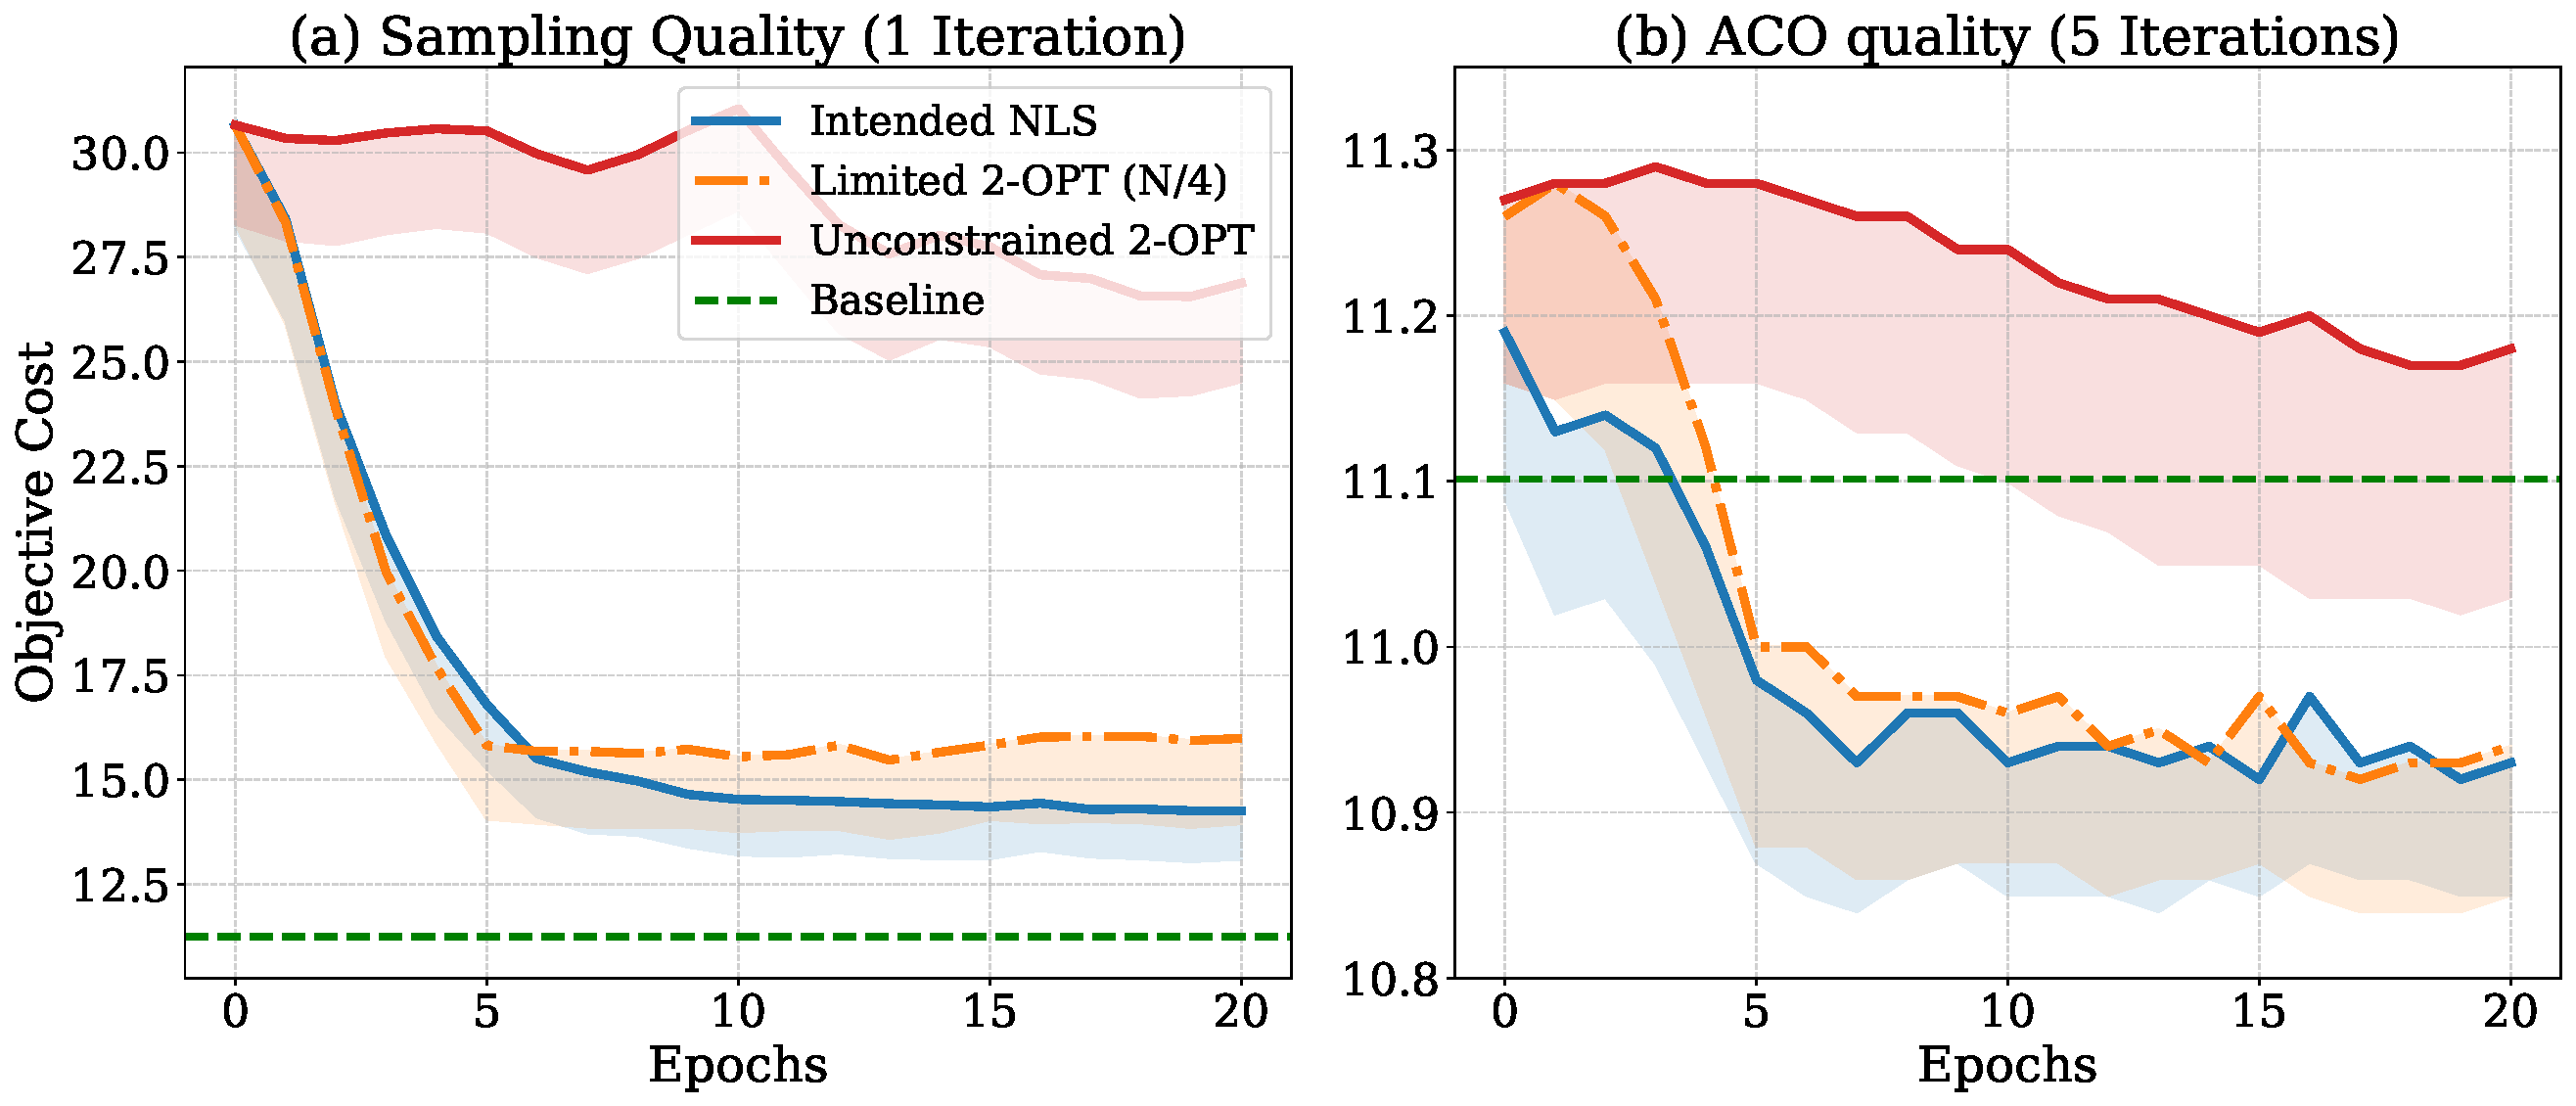
\includegraphics[width=\columnwidth]{figures/nls_vs_limited_vs_unconstrained.pdf}
    \caption{Credit-assignment trade-off under different local-search strategies when training DeepACO on TSP-200.}
    \label{fig:credit_assignment}
\end{figure}

Scalability imposes an additional constraint. Standard 2-opt costs $\mathcal{O}(N^2)$ per tour, which is prohibitive when refinement must be applied to every ant at every iteration. Classical large-scale ACO methods~\cite{partialACO, P-ACO} reduce this cost by applying local search only occasionally or only to elite ants. This is unsuitable for policy-gradient training, where per-ant advantages require post-refinement costs for all sampled ants. Thus, the refinement operator must satisfy three requirements simultaneously: it must preserve the causal link between policy actions and rewards, refine tours to convergence rather than stop at an arbitrary budget, and have cost independent of the full instance size.

We satisfy these requirements using Scope-Restricted Refinement (SRR), inspired by~\cite{faco}. The key observation is that perturbation-based ants start from an incumbent solution that is already locally optimized under the candidate graph. Since an ant modifies only a small set of edges, any newly introduced sub-optimality is localized around those interventions. SRR therefore acts as a local projection operator: it initializes a checklist with the endpoints of the perturbed edges and repeatedly applies improving candidate-graph refinement moves involving checked nodes, reactivating affected neighbors after each accepted move. In routing, these refinement moves are instantiated with candidate-limited 2-opt for \TSP{} and capacity-preserving relocate/swap/2-opt* operators for \CVRP{}; Appendix~\ref{app:setup} gives the algorithmic details. Conceptually, SRR propagates repair outward from the intervention region until no improving move remains within its scope.

Specifically, SRR provides the three properties required for training. First, because refinement is restricted to the neighborhood of the policy's perturbations, the post-refinement cost remains causally tied to the sampled actions, preserving credit assignment. Second, unlike truncated local search, SRR runs to convergence within its scope; assuming the incumbent was already candidate-graph 2-opt optimal, this restores candidate-graph 2-opt optimality after the perturbation. Third, the refinement cost scales with the perturbation size, $\mathcal{O}(M \cdot K)$, rather than the instance size, $\mathcal{O}(N^2)$, allowing SRR to be applied to every ant at every iteration even at $N{=}100$K.

% \smallskip\noindent\textbf{Scope-Restricted Refinement.}
% \label{sec:localized-ls} Other than the scalability, integrating local search (LS) into policy-gradient training presents another challenge: \emph{gradient washout}. If a powerful LS drastically rewrites the entire tour, it severs the causal link between the policy's initial decisions and the final rewards, destroying the learning signal. Figure~\ref{fig:credit_assignment} tracks the training progression of DeepACO on TSP-200 under three distinct LS strategies. When employing an \emph{Unconstrained 2-OPT} (red curve), the policy completely fails to converge. Because the unrestricted heuristic heavily rewrites the ant's initial tour, the causal link is thus severed. DeepACO attempts to mitigate this via \emph{Limited 2-OPT ($N/4$)} (orange curve); this restores the gradient signal but bottlenecks solution quality due to early stopping. Alternatively, its \emph{Intended NLS} (blue curve) achieves the lowest cost by using the neural policy to evaluate every candidate swap; however, this severely limits scalability by requiring $\mathcal{O}(N \cdot K)$ neural forward passes inside the refinement loop.
% The computational burden is exacerbated at scale: standard 2-opt costs $O(N^2)$ per tour, prohibitive for every ant on every iteration at $N{=}100$K. Classical large-scale ACO~\cite{partialACO, P-ACO} mitigates this by applying LS \emph{sparingly} (every few iterations) and \emph{elitely} (only to the best or top-$k$ ants), but policy-gradient training is incompatible: per-ant advantages require post-LS costs for \emph{every} ant at \emph{every} iteration. Capping swaps at a fixed budget reduces cost at the expense of quality, and the cap still scales with $N$ rather than the perturbation size.

% \begin{figure}[t]
%     \centering
%     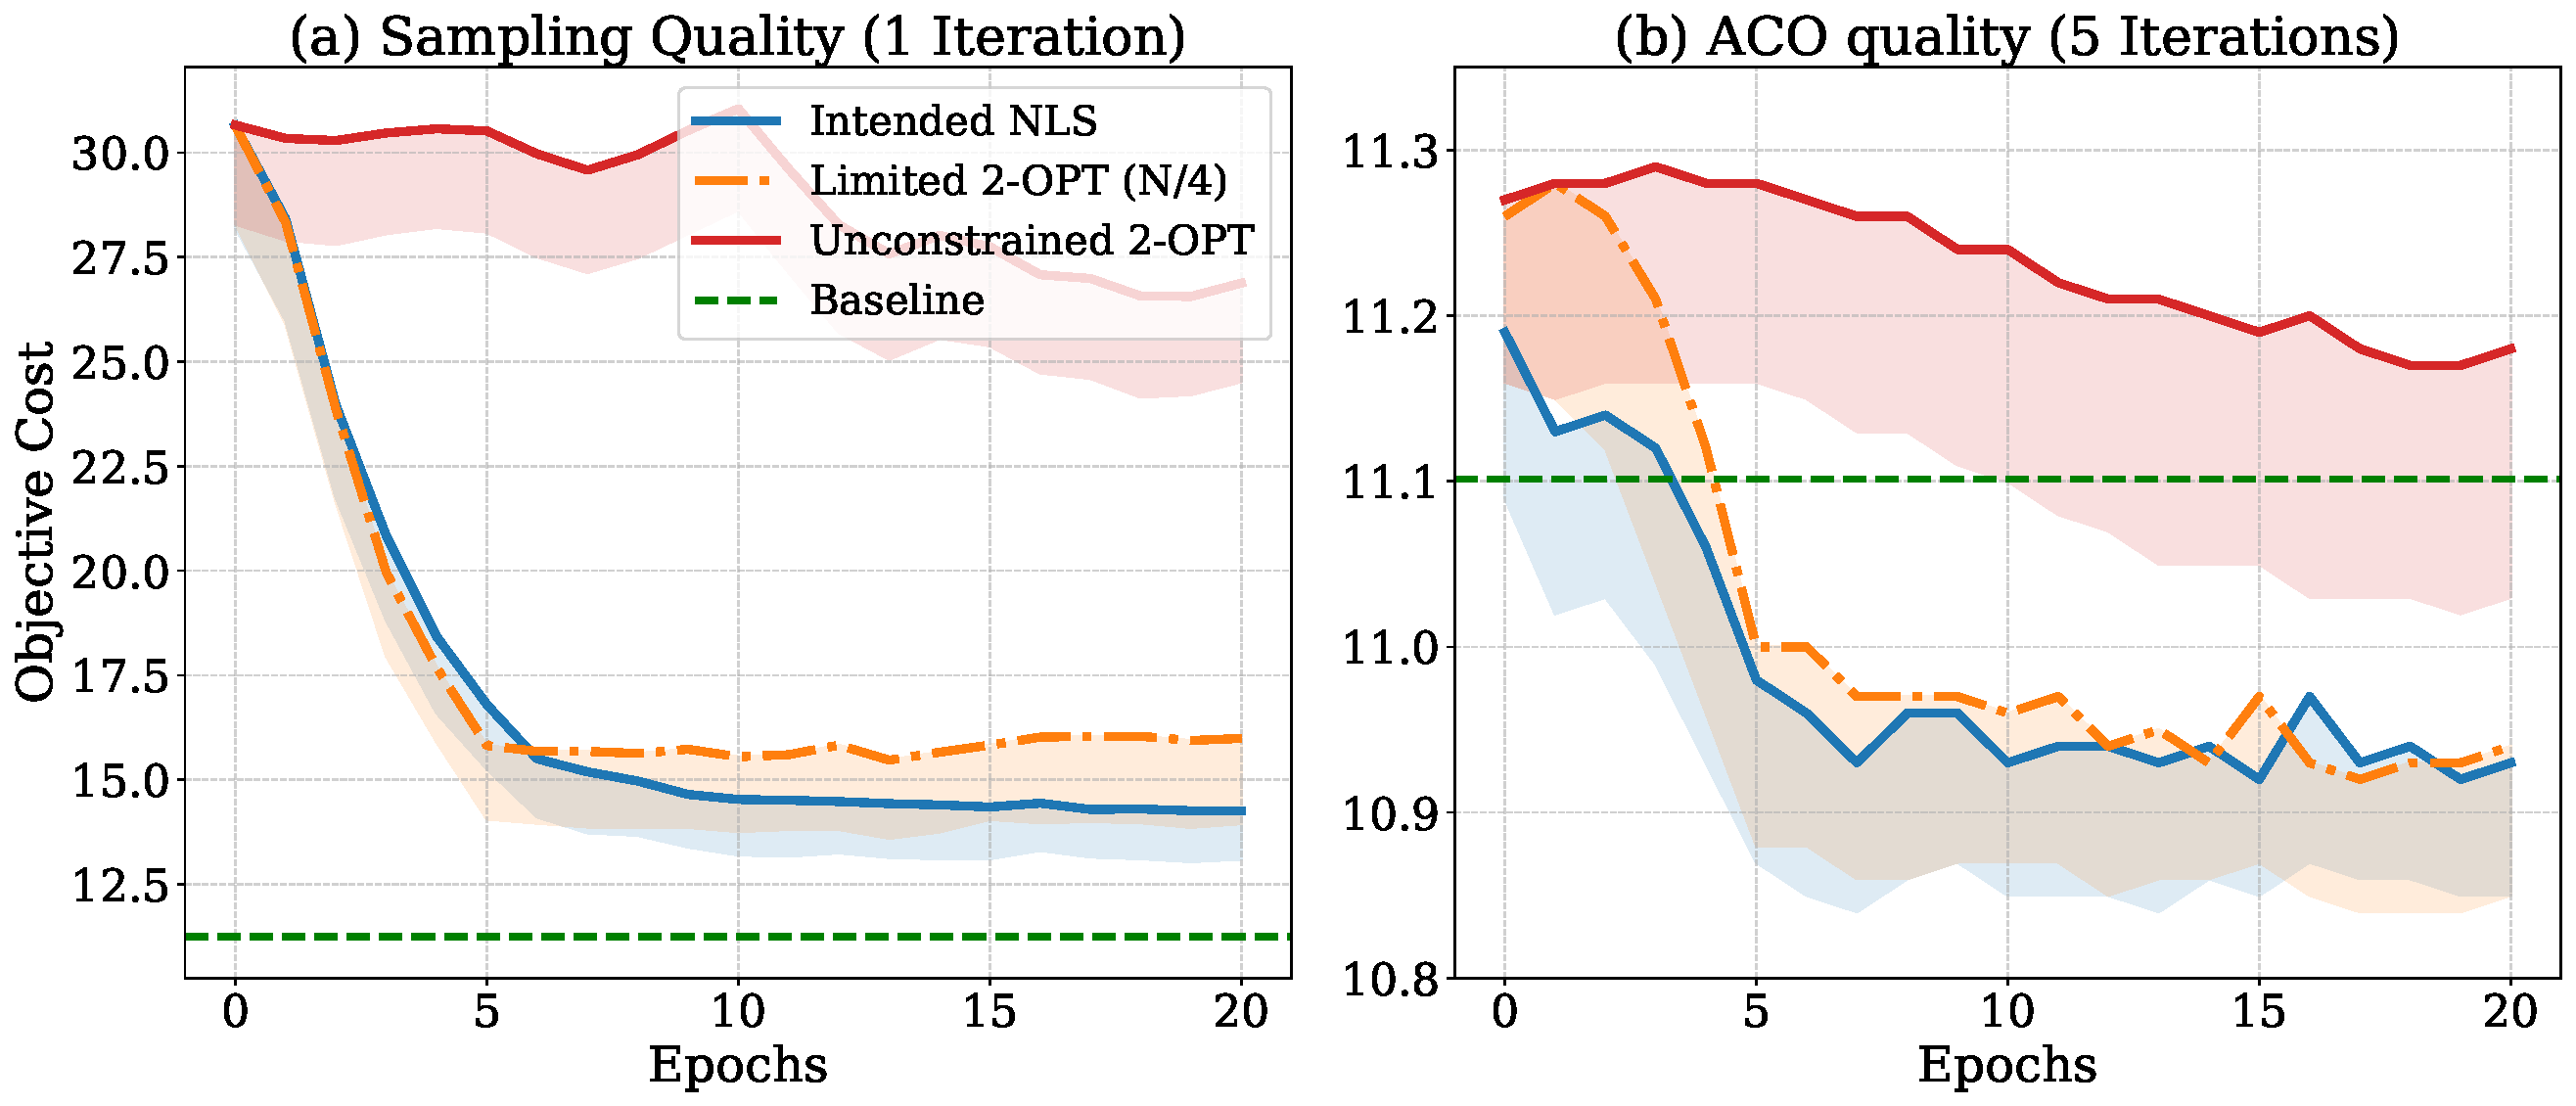
\includegraphics[width=\columnwidth]{figures/nls_vs_limited_vs_unconstrained.pdf}
%     \caption{The gradient washout trade-off: three LS strategies for training DeepACO on TSP-200.}
%     \label{fig:credit_assignment}
% \end{figure}

% We resolve this dilemma using Scope-Restricted Refinement (SRR)~\cite{faco}. The key insight is that the incumbent solution is generally already locally optimal.
% When an ant perturbs this solution, it creates a localized region of sub-optimality.
% SRR operates as a targeted repair mechanism, conceptually similar to a Breadth-First Search (BFS), that propagates improvements outward from the perturbed edges only.
% Unlike DeepACO's truncation strategy, SRR runs to convergence within its scope.
% Because the unperturbed regions of the tour were already optimized under the candidate graph, repairing the perturbed region restores 2-opt optimality with respect to the candidate-graph move set. SRR simultaneously provides three properties that existing designs achieve only in isolation:
% \begin{enumerate}
%     \item \emph{Stable Credit Assignment}: confining refinement to the neighborhood of the policy's actions preserves the causal link between neural decisions and rewards, matching NLS's credit-assignment role without additional neural forward passes.
%     \item \emph{Within-Scope Convergence}: unlike truncated LS, SRR runs to convergence, yielding a tour that is 2-opt optimal on the candidate-graph move set within the perturbed region.
%     \item \emph{Size-Independent Scalability}: refinement cost scales as $O(M{\cdot}K)$ with the perturbation size, not $O(N^2)$ with instance size, so SRR can be applied to \emph{every} ant at \emph{every} iteration (a requirement for policy-gradient training) even at $N{=}100$K.
% \end{enumerate}
% SRR thus combines the efficiency of truncated LS with the credit-assignment benefit of NLS: by guaranteeing that unperturbed regions remain locally optimal, convergent refinement within the perturbation scope is both sufficient and inexpensive (formal optimality argument in Section~\ref{app:credit}).

\smallskip\noindent\textbf{Stabilized Pheromone Dynamics.}
\label{sec:smoothed-mmas}
\MMAS{}~\cite{maxmin} bounds pheromones to $[\tau_{\min}, \tau_{\max}]$ to prevent premature convergence, but couples these bounds to solution cost, creating non-stationary input distributions for the state-aware policy. We instead adopt fixed bounds ($\tau_{\max}{=}1$, $\tau_{\min}{=}1/K$) and update via convex interpolation:
\begin{equation}
\tau^{(h,s+1)}_{ij} \leftarrow (1-\rho)\tau^{(h,s)}_{ij} + \rho \cdot \mathcal{T}_{ij},
\label{eq:smoothed-mmas}
\end{equation}
where $\mathcal{T}_{ij} = \tau_{\max}$ if $(i,j)$ is in the best solution, else $\tau_{\min}$.
This yields scale-invariant state representations and stabilizes training.
While this simplification may reduce the solution quality of the \emph{unguided} solver compared to highly tuned \MMAS{} dynamics, our ablations (Section~\ref{sec:ablations}) show that \DyNACO{} with stabilized bounds outperforms both (i)~unguided ACO with standard \MMAS{} updates and (ii)~neural-guided ACO retaining the original update rule.

\subsection{Inference Controls}
\label{sec:inference}
We use constant guidance ($\gamma{=}1$) during training, with no annealing or phased scheduling.
At inference, the guidance weight~$\gamma$ (Eq.~\ref{eq:held-logits}) can be modulated via two strategies: \emph{guidance annealing}, which linearly decays $\gamma \to 0$ across inner iterations; and \emph{phased injection}, which withholds neural guidance for the first fraction of outer steps.
The specific configuration varies by problem and scale: for TSP, we apply annealing at all scales and additionally enable phased injection at TSP-1K; for CVRP, we apply phased injection only at longer iteration budgets ($I{\geq}5000$) and never anneal.

\subsection{Cost and Memory Scaling}
\label{sec:complexity}

The computational cost separates into sparse neural inference and ACO operations based on perturbations. The GNN encoder runs once per outer step on the $K$-NN graph, giving $\mathcal{O}(H L n K d)$ neural cost for $H$ guidance updates, $L$ layers, $n$ nodes, $K$ candidates, and hidden dimension $d$. During the ACO search, each of the $m$ ants performs at most $M$ stochastic interventions, and SRR scans only the affected candidate neighborhoods. Over $T=H S$ inner iterations, this gives $\mathcal{O}(T m M K)$ sampling and local projection cost.

The learned state and replay buffers are also sparse. Pheromone snapshots, edge features, feasible masks, and action traces are stored on the candidate graph, requiring $\mathcal{O}(nK)$ memory rather than $\mathcal{O}(n^2)$ dense heatmaps. The extension from \DyNACO{} to \DyNACS{} reuses the same encoder and adds only lightweight behavior maps. This cost profile is what allows neural guidance to remain active during large search runs instead of being used only as an initialization heuristic.


% ======================================================================
% 5. Experiments and Analysis
% ======================================================================
\section{Experiments and Analysis}
\label{sec:experiments}

We evaluate \DyNACS{} as a zero-shot learning-guided optimizer within each problem type. Unless otherwise specified, a single model trained on uniformly distributed 1K-node synthetic instances is directly tested on benchmark \TSP{} and \CVRP{} instances with different scales, structures, and distributions. Conventional neural combinatorial optimization often trains and tests on matched synthetic distributions, or trains different models for different scales. Our evaluation instead asks whether state-aware guidance transfers beyond the training distribution while preserving the efficiency and reliability of the underlying ACO search.

The evaluation follows the method's dependency chain. The main benchmark comparison tests whether the full model improves zero-shot performance against classical solvers, neural routing solvers, and neural-guided ACO baselines. The trajectory-diversity study asks whether population-aware guidance improves the state-aware \DyNACO{} base model inside the same ACO environment. The ablations test dynamic guidance, SRR credit assignment, pheromone stabilization, and inference controls. The final analyses report runtime, neural overhead, training efficiency, and learned guidance behavior to clarify how the method scales in practice.

\subsection{Experimental Setup}
\label{sec:setup}

\smallskip\noindent\textbf{Training setup.}
All experiments use a fixed random seed and one deterministic run per instance. Training instances are generated online, with coordinates sampled uniformly from $[0,1]^2$, yielding 320 training instances in total (32 per epoch $\times$ 10 epochs). We train with PPO on a single RTX 5090 GPU and Ryzen 9 7950X CPU with 16 cores. Default \DyNACS{} hyperparameters are summarized in Table~\ref{tab:hyperparams}, and baseline configurations are detailed in Appendix~\ref{app:setup}.

\smallskip\noindent\textbf{Benchmark datasets.}
For the main zero-shot evaluation, we follow a benchmark protocol designed to test generalization. The \TSP{} test suite includes instances from TSPLIB~\cite{tsplib}, National TSP~\cite{nationaltsp}, VLSI TSP~\cite{vlsitsp}, and the 8th DIMACS Implementation Challenge for TSP~\cite{dimacs8tsp}. These datasets cover geographic, industrial, clustered, and benchmark-generated structures. The \CVRP{} test suite includes instances from CVRPLIB~\cite{cvrplib}, including Set X and large-scale AGS instances~\cite{ags}. We include only standard Euclidean instances with available best-known solutions and without additional side constraints such as fixed edges, fixed route numbers, or duration limits.

The benchmark suite is substantially more challenging than synthetic testing on the training distribution. The training distribution contains only uniform 1K-node instances, whereas the test suite contains benchmark instances with diverse structures and scales. Strong performance on this suite indicates zero-shot transfer across both scale and distribution.

\smallskip\noindent\textbf{Candidate graph and backend.}
The candidate graph is a symmetric $K$-nearest-neighbor graph with $K{=}32$, with ties broken by node index. A backup list of 64 additional neighbors is maintained for fallback~\cite{ACOTSP-MF}. For \TSP{}, the backend follows the ACO design based on perturbations from~\cite{faco}. For \CVRP{}, we use a capacity-aware version of the same backend with scope-restricted refinement, described in Appendix~\ref{app:cvrp}.

\smallskip\noindent\textbf{Baselines.}
We compare with four groups of methods. First, we include simple construction heuristics, including Nearest Neighbor and Random Insertion. These baselines are important because recent evaluations of generalization show that many neural solvers can degrade below simple heuristics under benchmark distribution shift. Second, we include strong classical solvers, including LKH-3~\cite{lkhtsp,lkhcvrp} for \TSP{} and HGS~\cite{hgs} and AILS-II~\cite{ails2} for \CVRP{}. Third, we compare with representative neural routing solvers, including BQ~\cite{bq}, LEHD~\cite{lehd}, SIL~\cite{sil}, ICAM~\cite{icam}, ELG~\cite{elg}, INViT~\cite{invit}, L2R~\cite{l2r}, DGL~\cite{dgl}, ReLD~\cite{reld}, L2C-Insert~\cite{l2c}, H-TSP~\cite{htsp}, DACT~\cite{dact}, NeuOpt~\cite{neuopt}, DRHG~\cite{drhg}, and Fast T2T~\cite{fastt2t}. Finally, we compare with neural-guided ACO methods, including DeepACO~\cite{deepaco}, GFACS~\cite{gfacs}, GTG-ACO~\cite{gtgaco}, and HeatACO~\cite{heataco}.

We also include the unguided ACO backend as a direct ablation baseline. Because \DyNACO{}, \DyNACS{}, and the unguided backend share the same candidate graph, perturbation mechanism, refinement procedure, and search budget, this comparison isolates the contribution of neural guidance.

\smallskip\noindent\textbf{Metrics.}
We report three complementary metrics. \emph{Effectiveness} is measured by the average optimality gap to the best-known solution (BKS):
\begin{equation}
\mathrm{Gap} =
\frac{\mathrm{Obj.}-\mathrm{BKS}}{\mathrm{BKS}}
\times 100%.
\end{equation}
\emph{Efficiency} is measured by wall-clock inference time. \emph{Reliability} is measured by the number of successfully solved instances. A method is considered unsuccessful if it runs out of memory, times out, fails to produce a feasible solution, or suffers severe performance breakdown. Results are grouped into three scale ranges: $(0,1\mathrm{K})$, $[1\mathrm{K},10\mathrm{K})$, and $[10\mathrm{K},100\mathrm{K}]$, with aggregate results also reported.

\subsection{Zero-Shot Generalization on Benchmarks}
\label{sec:main-results}

Table~\ref{tab:exp_proposed} presents the main zero-shot results on \TSP{} and \CVRP{} benchmarks. Unlike the conventional setting where training and testing distributions are matched, all neural methods are evaluated without retraining or fine-tuning on benchmark instances. \DyNACS{} achieves the strongest overall performance among neural methods while solving all instances.

\begin{table}[h]
\centering
\caption{Headline zero-shot results from Table~\ref{tab:exp_proposed}.}
\label{tab:headline-results}
\small
\renewcommand{\arraystretch}{0.85}
\begin{tabular*}{\columnwidth}{@{\extracolsep{\fill}}lcc@{}}
\toprule
Method & \TSP{} Total & \CVRP{} Total \\
\midrule
Best prior neural baseline & 1.71\% / 228 & 4.58\% / 107 \\
ACO backend & 1.82\% / 228 & 3.18\% / 110 \\
\DyNACO{} (single behavior) & 1.48\% / 228 & 3.10\% / 110 \\
\DyNACS{} & \textbf{1.22\% / 228} & \textbf{2.80\% / 110} \\
\bottomrule
\end{tabular*}
\end{table}


\begin{table*}[htbp]
  \centering
  \caption{Experimental Results of the Proposed Evaluation Pipeline}
  \vspace{-0.2cm}
  \tabcolsep=0.185cm
  \begin{threeparttable}
    \begin{tabular}{c|l|ccc|ccc|ccc|cc}
    \toprule[0.5mm]
          & \multicolumn{1}{c|}{\multirow{2}[2]{*}{Method}} & \multicolumn{3}{c|}{(0,1K)} & \multicolumn{3}{c|}{[1K, 10K)} & \multicolumn{3}{c|}{[10K, 100K]} & \multicolumn{2}{c}{Total} \\
\cmidrule{3-13}          &       & Gap   & Time  & \multicolumn{1}{l|}{Solved} & Gap   & Time  & \multicolumn{1}{l|}{Solved} & Gap   & Time  & \multicolumn{1}{l|}{Solved} & Gap   & Solved \\
\cmidrule{1-13}    \multirow{26}[13]{*}{\rotatebox[origin=c]{90}{TSP}} & Nearest Neighbor & 25.29\% & 0.01s & 69/69 & 26.66\% & 0.29s & 109/109 & 25.01\% & 22.60s & 50/50 & 25.88\% &  {{228}/228} \\
          & Random Insertion & 10.60\% &  {{0.00s}} & 69/69 & 15.32\% &  {{0.05s}} & 109/109 & 16.37\% &  {{8.93s}} & 50/50 & 14.12\% &  {{228}/228} \\
          & LKH-3\phantom{$^{\downarrow}$} t=n/3, runs=1 & 0.00\% & 7.88s & 69/69 & 0.01\% & 631.34s & 109/109 & 0.08\% & 14600.50s & 50/50 & 0.03\% &  {{228}/228} \\
          & LKH-3$^{\downarrow}$ t=n/3, runs=1 & 0.00\% & 9.25s & 69/69 & 0.01\% & 600.36s & 109/109 & 0.05\% & 10800.24s & 50/50 &  {{0.02\%}} &  {{228}/228} \\
\cmidrule{2-13}          & BQ    & 5.00\% & 2.51s & 68/69 & 19.03\% & 22.74s & 92/109 & 52.00\% & 187.81s & 4/50  & 14.02\% & 164/228 \\
          & LEHD$^*$ greedy & 4.85\% & 1.01s & 69/69 & 20.13\% & 68.27s & 106/109 & 49.35\% & 1386.01s & 11/50 & 16.19\% & 186/228 \\
          & SIL$^*$ greedy & 8.64\% & 1.69s & 69/69 & 9.83\% & 17.69s & 109/109 & 11.11\% & 430.73s & 50/50 & 9.75\% &  {{228}/228} \\
          & ICAM  & 6.53\% & 0.25s & 69/69 & 16.62\% & 21.57s & 109/109 & 21.34\% & 1050.33s & 19/50 & 13.54\% & 197/228 \\
          & ELG   & 6.05\% & 0.63s & 69/69 & 18.14\% & 88.12s & 108/109 & 21.65\% & 940.35s & 6/50  & 13.70\% & 183/228 \\
          & INViT-3V   & 7.93\% & 2.77s & 69/69 & 12.08\% & 49.03s & 109/109 & 11.52\% & 1079.50s & 42/50 & 10.67\% & 220/228 \\
          & L2R   & 5.89\% & 1.60s & 69/69 & 9.22\% & 15.55s & 109/109 & 8.52\% & 153.11s & 50/50 &  {{8.06\%}} &  {{228}/228}   \\
          & DGL   & 6.53\% & 1.17s & 69/69 & 11.32\% & 11.67s & 109/109 & 11.14\% & 58.62s & 25/50 & 9.67\% & 203/228 \\
          & L2C-Insert$^*$ greedy & 4.39\% & 1.51s & 69/69 & 18.12\% & 15.34s & 109/109 & 30.94\% & 145.17s & 50/50 & 16.77\% &  {{228}/228}   \\
\cmidrule{2-13}          & H-TSP & 6.16\% &  {{0.61s}} & 36/69 & 11.62\% &  {{3.15s}} & 100/109 & 12.29\% &  {{21.44s}} & 40/50 & 10.65\% & 176/228 \\
\cmidrule{2-13}          & DACT T=1K & 16.37\% & 39.84s & 69/69 & 26.58\% & 261.73s & 83/109 & /     & /     & 0/50  & 21.94\% & 152/228 \\
          & NeuOpt T=1K & 19.90\% & 81.22s & 46/69 & /     & /     & 0/109 & /     & /     & 0/50  & 19.90\% & 46/228 \\
\cmidrule{2-13}          & L2C-Insert$^*$ T=1K & 1.08\% & 381.55s & 69/69 & 9.80\% & 479.98s & 109/109 & 29.15\% & 615.19s & 50/50 & 11.41\% &  {{228}/228}   \\
          & LEHD$^*$ RRC1K & 1.73\% & 498.40s & 69/69 & 10.87\% & 1634.51s & 109/109 & 24.02\% & 2769.86s & 9/50  & 8.13\% & 187/228 \\
          & SIL$^*$ PRC1K & 0.80\% & 883.87s & 69/69 & 2.58\% & 2880.46s & 109/109 & 4.55\% & 4933.45s & 50/50 & 2.47\% &  {{228}/228} \\
          & DRHG T=1K & 0.10\% & 769.53s & 69/69 & 1.46\% & 2857.55s & 109/109 & 4.46\% & 3004.28s & 50/50 &  {{1.71\%}} &  {{228}/228}   \\
          & Fast T2T T\textsubscript{s}=10, T\textsubscript{g}=10 & 10.46\% & 1.41s & 45/69 & /     & /     & 0/109 & /     & /     & 0/50  & 10.46\% & 45/228 \\
\cmidrule{2-13}          & GFACS$^{\dagger}$ T=100, K=100 & 31.64\% & 166.94s & 66/69 & 86.77\% & 2601.13s & 22/109 & /     & /     & 0/50  & 45.42\% & 88/228 \\
          & GFACS$^{\ddagger}$ T=100, K=100 & 0.72\% & 174.21s & 69/69 & 3.76\% & 9142.93s & 83/109 & /     & /     & 0/50  & 2.38\% & 152/228 \\
    \midrule

\cmidrule{2-13}
          & ACO
          & 0.28\% & -- & 69/69
          & 1.59\% & -- & 109/109
          & 4.44\% & -- & 50/50
          & 1.82\% & 228/228 \\

          & \DyNACO{}
          & 0.23\% & 0.59s & 69/69
          & 1.22\% & 1.58s & 109/109
          & 3.99\% & 12.14s & 50/50
          & 1.48\% & 228/228 \\

          & \DyNACS{}
          & \textbf{0.14\%} & 0.86s & \textbf{69/69}
          & \textbf{0.95\%} & 3.39s & \textbf{109/109}
          & \textbf{3.33\%} & 34.45s & \textbf{50/50}
          & \textbf{1.22\%} & \textbf{228/228} \\


\midrule
    \midrule
    \multirow{25}[13]{*}{\rotatebox[origin=c]{90}{CVRP}} & Nearest Neighbor & 21.17\% & 0.03s & 99/99 & 15.18\% & 1.08s & 5/5   & 11.80\% & 14.63s & 6/6   & 20.39\% &  {{110}/110} \\
          & Random Insertion & 75.00\% & 0.00s & 36/99 & /     & /     & 0/5   & /     & /     & 0/6   & 75.00\% & 36/110 \\
          & HGS t=n/3 & 0.29\% & 111.24s & 99/99 & 3.59\% & 1428.41s & 5/5   & 7.86\% & 6926.41s & 6/6   & 0.85\% &  {{110}/110} \\
          & AILS-II t=n/3 & 0.57\% & 133.95s & 99/99 & 1.58\% & 1388.42s & 5/5   & 1.58\% & 5646.48s & 6/6   &  {{0.68\%}} &  {{110}/110} \\
\cmidrule{2-13}          & BQ   & 8.87\% & 3.63s & 99/99 & 20.28\% & 39.97s & 5/5   & 41.52\% & 202.69s & 5/6   & 10.89\% & 109/110 \\
          & LEHD$^*$ greedy & 11.25\% & 1.53s & 98/99 & 19.22\% & 99.43s & 5/5   & 32.80\% & 852.02s & 2/6   & 12.04\% & 105/110 \\
          & SIL$^*$ greedy & 40.04\% & 2.48s & 65/99 & 16.09\% & 26.86s & 5/5   & 10.81\% & 146.83s & 6/6   & 36.16\% & 76/110 \\
          & ICAM  & 5.00\% & 0.42s & 99/99 & 11.69\% & 32.32s & 5/5   & /     & /     & 0/6   & 5.32\% & 104/110 \\
          & ELG   & 8.03\% & 1.29s & 99/99 & 18.51\% & 30.21s & 5/5   & 29.38\% & 133.08s & 2/6   & 8.93\% & 106/110 \\
          & INViT-3V   & 13.15\% & 4.72s & 99/99 & 19.03\% & 77.33s & 5/5   & 23.91\% & 496.25s & 5/6   & 13.91\% & 109/110 \\
          & L2R   & 8.16\% & 2.49s & 99/99 & 11.62\% & 23.99s & 5/5   & 11.08\% & 97.12s & 6/6   & 8.48\% &  {{110}/110}   \\
          & DGL   & 15.27\% & 2.22s & 99/99 & 17.96\% & 22.60s & 5/5   & 18.69\% & 78.64s & 5/6   & 15.55\% & 109/110 \\
          & ReLD  & 4.10\% & 0.41s & 99/99 & 10.22\% & 5.29s & 5/5   & 11.27\% & 28.87s & 3/6   &  {{4.58\%}} & 107/110 \\
          & L2C-Insert$^*$ greedy & 6.87\% & 2.73s & 99/99 & 22.37\% & 616.75s & 5/5   & 49.41\% & 5525.71s & 2/6   & 8.40\% & 106/110 \\
\cmidrule{2-13}          & DACT T=1K & 16.42\% & 246.51s & 74/99 & 17.70\% & 479.82s & 1/5   & /     & /     & 0/6   & 16.44\% & 75/110 \\
          & NeuOpt T=1K & 26.93\% & 571.14s & 36/99 & /     & /     & 0/5   & /     & /     & 0/6   & 26.93\% & 36/110 \\
\cmidrule{2-13}          & L2C-Insert$^*$ T=1K & 3.21\% & 344.05s & 99/99 & 18.87\% & 6166.21s & 5/5   & 44.29\% & 32754.86s & 2/6   & 4.72\% & 106/110 \\
          & LEHD$^*$ RRC1K & 3.58\% & 796.15s & 99/99 & 11.73\% & 2043.74s & 5/5   & 21.98\% & 2820.28s & 2/6   & 4.32\% & 106/110 \\
          & SIL$^*$ PRC1K  & 21.38\% & 1307.97s & 99/99 & 8.28\% & 3471.69s & 5/5   & 7.40\% & 4251.88s & 6/6   & 20.02\% &  {{110}/110}   \\
          & DRHG T=1K & 11.11\% & 1114.60s & 99/99 & 17.95\% & 2529.12s & 5/5   & 16.95\% & 5376.37s & 6/6   & 11.74\% &  {{110}/110}   \\
\cmidrule{2-13}          & GFACS$^{\dagger}$ T=100, K=100 & 36.83\% & 437.38s & 99/99 & 34.09\% & 9654.33s & 3/5   & /     & /     & 0/6   & 36.75\% & 102/110 \\
          & GFACS$^{\ddagger}$ T=100, K=100 & 2.60\% & 405.81s & 99/99 & 7.65\% & 14884.94s & 4/5   & /     & /     & 0/6   & 2.80\% & 103/110 \\
    \midrule

\cmidrule{2-13}
          & ACO
          & 2.83\% & -- & 99/99
          & 5.33\% & -- & 5/5
          & 7.16\% & -- & 6/6
          & 3.18\% & 110/110 \\

          & \DyNACO{}
          & 2.77\% & 1.64s & 99/99
          & 5.01\% & 7.50s & 5/5
          & 6.98\% & 27.64s & 6/6
          & 3.10\% & 110/110 \\

          & \DyNACS{} (ours)
          & \textbf{2.42\%} & -- & \textbf{99/99}
          & \textbf{4.82\%} & -- & \textbf{5/5}
          & \textbf{6.98\%} & -- & \textbf{6/6}
          & \textbf{2.80\%} & \textbf{110/110} \\



    \bottomrule[0.5mm]
    \end{tabular}%
    \begin{tablenotes}
      \footnotesize
      \item[$\downarrow$] $Initial\_Period$ is set as 1K, rather than the original value DIMENSION/2.
      \item[$*$]  The NRS supports more than one inference strategy.
      \item[$\dagger$] GFACS without local search at the last generation. The output solution is the best of the population at the last generation.
      \item[$\ddagger$] The original version of GFACS\@. The output solution is the best in history (all after local search). 
      
    \end{tablenotes}
    \end{threeparttable}
    \vspace{-0.6cm}
  \label{tab:exp_proposed}%
\end{table*}%

\smallskip\noindent\textbf{TSP.}
On \TSP{}, \DyNACS{} achieves the best aggregate gap among neural methods while solving all 228 instances. The advantage is most visible in the medium and large groups, where several end-to-end neural solvers lose instances or degrade sharply. Against the shared ACO backend, the gain is smaller but consistent, showing that learned guidance improves the same search environment under the matched evaluation budget.

\smallskip\noindent\textbf{CVRP.}
On \CVRP{}, \DyNACS{} also gives the best aggregate neural result and solves all 110 instances. The gain over the ACO backend is larger than on \TSP{} in the total column, consistent with the role of multiple learned behaviors in capacity-constrained search, where local decisions are more heterogeneous. \DyNACS{} improves quality while preserving full reliability.

\smallskip\noindent\textbf{Comparison with simple heuristics.}
Nearest Neighbor and Random Insertion test whether neural methods provide value beyond simple handcrafted rules. \DyNACS{} substantially outperforms these heuristics on both problems while preserving full reliability. Several neural baselines degrade below simple heuristics under benchmark distribution shift, highlighting the gap between synthetic-distribution performance and zero-shot benchmark deployment.

\smallskip\noindent\textbf{Scalability of neural baselines.}
The failures and high runtimes of several neural baselines are largely explained by their inference structure. End-to-end constructive policies~\cite{attentionmodel,pomo,bq,lehd,invit,sigd} are usually trained on small instances and often rely on quadratic attention in the number of nodes. When applied directly to larger benchmarks, they face both scale shift and memory pressure. Neural ACO baselines encounter a related dense bottleneck because they materialize heatmap or pheromone-prior matrices in $\mathbb{R}^{N\times N}$ and then use them inside an ACO loop. Decomposition and hierarchical methods such as GLOP~\cite{glop}, H-TSP~\cite{htsp}, SIL~\cite{sil}, and LEHD~\cite{lehd} mitigate this issue, but their global context modules or repeated subproblem calls can still become expensive at extreme scales. In contrast, \DyNACS{} keeps both neural inference and search state on a sparse $K$-NN graph, so the learned component scales with $nK$ rather than a dense edge matrix.

\smallskip\noindent\textbf{Comparison with classical solvers.}
Classical solvers such as LKH-3, HGS, and AILS-II remain stronger in absolute solution quality, reflecting decades of specialized engineering. The learning question in this paper is whether a neural policy can improve a scalable ACO backend under zero-shot evaluation. Table~\ref{tab:exp_proposed} shows consistent gains while keeping reliability at 100\% on both problem families.

\subsection{Effect of Trajectory-Diverse Guidance}
\label{sec:trajectory-diverse-effect}

Table~\ref{tab:trajectory-diverse-effect} compares the three stages of the search system under the same backend and budget. The unguided backend gives the shared ACO environment. \DyNACO{} adds state-aware guidance, reducing the static-heatmap mismatch by updating the transition prior from the current pheromone and incumbent state. \DyNACS{} keeps the same dynamic state representation and lets different ant groups follow behavior-conditioned trajectory distributions in the same colony. The additional reduction from \DyNACO{} to \DyNACS{} connects the improvement to population-level diversity within the observed search state.

\begin{table}[h]
\centering
\caption{Aggregate zero-shot effect of trajectory-diverse guidance from Table~\ref{tab:exp_proposed}.}
\label{tab:trajectory-diverse-effect}
\small
\renewcommand{\arraystretch}{0.85}
\begin{tabular*}{\columnwidth}{@{\extracolsep{\fill}}lcc@{}}
\toprule
Method & \TSP{} Gap & \CVRP{} Gap \\
\midrule
ACO backend & 1.82\%  & 3.18\%  \\
\DyNACO{} (single behavior) & 1.48\% & 3.10\%  \\
\DyNACS{} & \textbf{1.22\%}  & \textbf{2.80\%} \\
\bottomrule
\end{tabular*}
\end{table}

\subsection{Zero-Shot Comparison with Neural-Guided ACO}
\label{sec:neural-aco-comparison}

Table~\ref{tab:neural-aco} compares \DyNACS{} with prior neural-guided ACO methods at their maximum reported scales. Existing neural ACO methods mainly use static heatmaps or static heuristic priors. \DyNACS{} updates guidance throughout the search trajectory and keeps several learned transition priors active inside one shared colony. The comparison supports the central claim that neural guidance should interact with the ACO trajectory as it unfolds, both through state adaptation and through population-level search diversity.


\begin{table}[h]
\centering
\small
\renewcommand{\arraystretch}{0.85}
\caption{Comparison with neural-guided ACO methods at their maximum reported scale. HeatACO~\cite{heataco} combines ACO with other pretrained heatmap models~\cite{attgcn, dimes, utsp, difusco}.}
\label{tab:neural-aco}
\resizebox{\columnwidth}{!}{%
\begin{tabular}{lcccccc}
\toprule
& \multicolumn{2}{c}{\TSP{}1K} & \multicolumn{2}{c}{\TSP{}10K} & \multicolumn{2}{c}{\CVRP{}1K} \\
\cmidrule(lr){2-3} \cmidrule(lr){4-5} \cmidrule(lr){6-7}
Method & Gap & Time & Gap & Time & Gap & Time \\
\midrule
DeepACO~\cite{deepaco}       & 2.87\% & 66s & -- & -- & 2.40\% & 1.3m \\
GFACS~\cite{gfacs}           & 2.63\% & 66s & -- & -- & 2.11\% & 1.3m \\
GTG-ACO~\cite{gtgaco}        & 2.42\% & -- & -- & -- & -- & -- \\
\midrule
ACO+AttGCN~\cite{attgcn}    & 0.44\% & 5s & 1.27\% & 1.47m & -- & -- \\
ACO+DIMES~\cite{dimes}     & 0.39\% & 6s & 1.15\% & 1.4m & -- & -- \\
ACO+UTSP~\cite{utsp}      & 0.42\% & 6s & -- & -- & -- & -- \\
ACO+DIFUSCO~\cite{difusco}   & 0.23\% & 10s & 1.19\% & 2.89m & -- & -- \\
\midrule
\textbf{\DyNACS{} (ours)}                & \textbf{0.20\%} & 4s & \textbf{0.82\%} & 18s & \textbf{1.04\%} & 19s \\
\bottomrule
\end{tabular}}
\end{table}

\subsection{Credit Assignment and Component Ablations}
\label{sec:ablations}

\smallskip\noindent\textbf{Both dynamic guidance mechanisms are essential.}
Table~\ref{tab:ablation-decoupling} separates the two core parts of dynamic neural guidance. Removing training over full trajectories causes the largest degradation, especially on \TSP{}1K and \TSP{}5K. Removing the representation of the search state also hurts performance across all four columns. The ordering of the rows suggests that trajectory-aware training supplies the larger gain, while state features provide an additional improvement once the policy is trained on full search trajectories.

\begin{table}[h]
\centering
\caption{Decoupling the two mechanisms of dynamic neural guidance. Values are gap (\%) to BKS on 16 instances at I$_{1000}$.}
\label{tab:ablation-decoupling}
\small
\resizebox{\columnwidth}{!}{%
\begin{tabular}{lcccc}
\toprule

Method & TSP1K $\downarrow$ & TSP5K $\downarrow$ & TSP10K $\downarrow$ & CVRP1K $\downarrow$ \\
\midrule
Static only       & 3.65 & 4.87 & 3.56 & 3.00 \\
+ Trajectory-aware Training   & 0.75 & 2.11 & 2.28 & 2.79 \\
+ State-aware Representation  (Full)     & \textbf{0.37} & \textbf{1.24} & \textbf{1.62} & \textbf{2.58} \\
\bottomrule
\end{tabular}
}
\end{table}

\smallskip\noindent\textbf{SRR preserves both training signal and search quality.}
Tables~\ref{tab:srr-training} and~\ref{tab:srr-inference} compare SRR with full local search (FLS) and truncated local search (TLS). FLS can produce strong individual solutions, but it may rewrite the sampled perturbation enough to wash out the model's contribution. TLS preserves more of the policy signal, but leaves solutions under-refined. SRR provides the best trade-off: it runs local search to convergence within the perturbation scope, preserving the causal link between the policy action and the post-refinement reward while maintaining low refinement cost.

\begin{table}[h]
\centering
\caption{Training progress under different refinement strategies. Values are improvement over the untrained model.}
\label{tab:srr-training}
\small
\setlength{\tabcolsep}{0pt}
\renewcommand{\arraystretch}{0.80}
\begin{tabular*}{\columnwidth}{@{\extracolsep{\fill}}lccc@{}}
\toprule
Epoch & SRR $\uparrow$ & TLS $\uparrow$ & FLS $\uparrow$ \\
\midrule
0 (untrained) & 0.000\% & 0.000\% & 0.000\% \\
1 & \textbf{+0.224\%} & +0.099\% & -0.003\% \\
5 & \textbf{+0.432\%} & +0.146\% & -0.016\% \\
9 & \textbf{+0.438\%} & +0.127\% & -0.023\% \\
\midrule
Avg. ACO time & \textbf{2.35s} & 4.33s & 8.03s \\
\bottomrule
\end{tabular*}
\end{table}

\begin{table}[h]
\centering
\caption{Inference quality and runtime under different refinement strategies (TSP-5K, I$_{1000}$).}
\label{tab:srr-inference}
\small
\renewcommand{\arraystretch}{0.85}
\begin{tabular*}{\columnwidth}{@{\extracolsep{\fill}}lccc@{}}
\toprule
Refinement & Time (s) & Obj. & Gap to LKH-3 \\
\midrule
FLS & 13.63 & 53.76 & 5.47\% \\
TLS & 7.62 & 57.80 & 13.39\% \\
SRR & \textbf{1.93} & \textbf{51.66} & \textbf{1.35\%} \\
\bottomrule
\end{tabular*}
\end{table}

\smallskip\noindent\textbf{Pheromone stabilization improves consistency without replacing dynamic guidance.}
Table~\ref{tab:ps-ablation} shows that pheromone stabilization improves the consistency of the training signal for both the unguided backend and \DyNACO{}. Dynamic guidance remains beneficial with or without stabilized pheromone bounds, while stabilization further improves the final guided solver.

\begin{table}[h]
\centering
\caption{Ablation of pheromone stabilization (PS). Values are gap (\%) to BKS.}
\label{tab:ps-ablation}
\small
\renewcommand{\arraystretch}{0.85}
\setlength{\tabcolsep}{2.5pt}
\begin{tabular*}{\columnwidth}{@{\extracolsep{\fill}}lcccc@{}}
\toprule
Dataset & \shortstack{ACO\\w/o PS} & \shortstack{\DyNACO{}\\w/o PS} & ACO & \DyNACO{} \\
\midrule
CVRP-1K & 4.09 & \textbf{3.51} & 2.94 & \textbf{2.50} \\
CVRPlib (5) & 2.91 & \textbf{2.71} & 2.76 & \textbf{2.18} \\
\bottomrule
\end{tabular*}
\end{table}

\smallskip\noindent\textbf{Inference-time strategies provide complementary gains.}
All models are trained identically on the full trajectory with constant $\gamma{=}1$. At inference, guidance annealing and phased injection are applied as fixed problem- and scale-level configurations, rather than tuned per instance. Table~\ref{tab:inference-config} reports the configurations, and Table~\ref{tab:ablation-inference} shows their effects. On \TSP{}, both strategies yield consistent improvements; on \CVRP{}, phased injection is mainly beneficial at longer horizons.

\begin{table}[h]
\centering
\caption{Inference strategy configuration per problem \& scale.}
\label{tab:inference-config}
\small
\renewcommand{\arraystretch}{0.85}
\begin{tabular*}{\columnwidth}{@{\extracolsep{\fill}}lcc@{}}
\toprule
Setting & Annealing & Phased Injection \\
\midrule
TSP-1K (all budgets)          & \checkmark & \checkmark \\
TSP-5K, 10K, 50K, 100K       & \checkmark &            \\
CVRP (all scales, $I{<}5000$) &            &            \\
CVRP (all scales, $I{\geq}5000$) &         & \checkmark \\
\bottomrule
\end{tabular*}
\end{table}

\begin{table}[h]
\centering
\caption{Inference strategy ablation with gap (\%) to BKS\@. All models trained with $\gamma{=}1$; strategies applied post-hoc.}
\label{tab:ablation-inference}
\footnotesize
\setlength{\tabcolsep}{2pt}
\begin{tabular*}{\columnwidth}{@{\extracolsep{\fill}}lcccc@{}}
\toprule
Strategy & \shortstack{TSP\\5K} & \shortstack{TSP\\10K} & \shortstack{CVRP\\5K} & \shortstack{CVRP\\10K} \\
\midrule
Constant ($\gamma{=}1$)            & 1.38 & 1.73 & \textbf{6.58} & 11.16 \\
Phased injection           & \textbf{1.20} & 1.68 & 7.07 & \textbf{10.86} \\
Guidance annealing         & 1.23 & \textbf{1.59} & 6.84 & 11.17 \\
Phased + Annealing         & 1.23 & 1.60 & 7.35 & 11.02 \\
\bottomrule
\end{tabular*}
\end{table}

Training and inference use different guidance schedules. During training, annealing the guidance weight would scale the policy gradient by $\gamma_t$ and weaken late-stage learning as $\gamma_t \to 0$; phased injection would similarly hide early pheromone states from the policy. We train with constant $\gamma{=}1$ over the full trajectory and apply annealing or phased injection only as post-hoc inference controls. On \TSP{}-5K, Table~\ref{tab:train-strategy} shows that training-time annealing or phasing gives no consistent advantage, while post-hoc inference controls recover the best results with one training regime.

\begin{table}[h]
\centering
\caption{Training regime vs.\ inference strategy on \TSP{}-5K ($I_{1000}$). Gap (\%) to BKS; lower is better.}
\label{tab:train-strategy}
\footnotesize
\setlength{\tabcolsep}{2pt}
\begin{tabular*}{\columnwidth}{@{\extracolsep{\fill}}lcccc@{}}
\toprule
Training Regime & Constant & Anneal & Phased & Phased+Anneal \\
\midrule
Constant $\gamma{=}1$ & 1.39 & \textbf{1.24} & \textbf{1.21} & 1.28 \\
Anneal $\gamma{\to}0$ & \textbf{1.31} & 1.35 & 1.23 & \textbf{1.23} \\
Phased ($\phi{=}0.5$) & 1.37 & 1.26 & 1.24 & 1.25 \\
\bottomrule
\end{tabular*}
\end{table}

\subsection{Sensitivity to Search Granularity}
\label{sec:sensitivity_summary}

\DyNACS{} is stable under moderate changes to the candidate graph and search granularity. Increasing the number of candidates $K$ improves solution quality with the expected near-linear runtime tradeoff, while perturbation length $M$ has a problem-dependent optimum because overly long interventions can disrupt the incumbent basin and increase refinement work. Varying the outer guidance updates $H$ and inner ACO steps $S$ while keeping the total iteration budget fixed produces small differences, which supports the fixed-duration semi-MDP abstraction used by the policy. Appendix~\ref{extended_ablation} reports the detailed sensitivity tables for $K$, $M$, $H$, and $S$.

\subsection{Efficiency and Neural Overhead}
\label{sec:runtime}

A practical learning-guided optimizer must improve solution quality without introducing prohibitive neural overhead. Table~\ref{tab:time-breakdown} compares the runtime of \DyNACS{} and the unguided ACO backend at matched iteration budgets.

\begin{table}[h]
\centering
\caption{Time breakdown (CPU vs.\ GPU) and quality for unguided ACO vs.\ \DyNACS{} at $I_{10000}$.}
\label{tab:time-breakdown}
\small
\renewcommand{\arraystretch}{0.80}
\resizebox{\columnwidth}{!}{%
\begin{tabular}{llcccc}
\toprule
Problem & Method & Gap & CPU (s) & GPU (s) & Total (s) \\
\midrule
\multirow{2}{*}{\TSP{}1K}
  & ACO    & 0.48\% & 5.44  & --   & 5.44  \\
  & \DyNACS{} & \textbf{0.20\%} & 3.52  & 0.16  & 3.68  \\
\midrule
\multirow{2}{*}{\TSP{}10K}
  & ACO    & 2.02\% & 26.81 & --   & 26.81 \\
  & \DyNACS{} & \textbf{0.82\%} & 16.79 & 1.10  & 17.89 \\
\midrule
\multirow{2}{*}{\TSP{}100K}
  & ACO    & 3.12\% & 223.32 & --    & 223.32 \\
  & \DyNACS{} & \textbf{1.90\%} & 159.85 & 11.84 & 171.69 \\
\midrule
\midrule
\multirow{2}{*}{\CVRP{}1K}
  & ACO    & 1.85\% & 20.17 & --   & 20.17 \\
  & \DyNACS{} & \textbf{1.04\%} & 18.88 & 0.17  & 19.05 \\
\midrule
\multirow{2}{*}{\CVRP{}10K}
  & ACO    & 6.76\% & 74.43 & --   & 74.43 \\
  & \DyNACS{} & \textbf{6.04\%} & 76.14 & 0.56  & 76.70 \\
\midrule
\multirow{2}{*}{\CVRP{}100K}
  & ACO    & 7.26\% & 692.81 & --   & 692.81 \\
  & \DyNACS{} & \textbf{6.75\%} & 696.04 & 5.93  & 701.97 \\
\bottomrule
\end{tabular}}
\end{table}


On \TSP{}, \DyNACS{} reduces total runtime at the reported scales while also improving solution quality. The CPU component decreases enough to offset the GPU inference cost, which is consistent with SRR requiring fewer repair steps after better-targeted perturbations. On \CVRP{}, the capacity-aware backend dominates runtime; the GPU column remains below 1\% of total time at larger scales, while the quality column still improves over the unguided backend.

\subsection{Training Efficiency}
\label{sec:training-efficiency}

\DyNACS{} converges in approximately 30 minutes for TSP-1K and roughly 4 hours for TSP-100K on our machine, using only 320 training instances. This is substantially lighter than many end-to-end neural solvers that require large offline datasets or long training schedules. The shared \DyNACO{} encoder keeps the parameter count essentially scale independent because the architecture operates on local $K$-NN neighborhoods; \DyNACS{} adds only lightweight behavior maps on top of this representation. Appendix~\ref{extended_ablation} reports the memory overhead of static and dynamic feature inputs in Table~\ref{tab:feature-memory-app}.

\subsection{Extension to Other COPs}
\label{sec:other-cops}

Table~\ref{tab:other-cops} evaluates whether the same dynamic guidance policy can extend beyond routing. We test on Orienteering, Multiple Knapsack, and Bin Packing using the same environments as~\cite{deepaco}. These experiments omit SRR, so the comparison focuses on dynamic guidance inside existing ACO algorithms. Dynamic guidance improves over both unguided ACO and static guidance on all three problems, suggesting that the learned guidance is not tied to a routing objective, even though SRR remains essential for large routing instances.

\begin{table}[h]
\centering
\caption{Extension to additional COPs. Higher is better.}
\label{tab:other-cops}
\small
\renewcommand{\arraystretch}{0.85}
\begin{tabular*}{\columnwidth}{@{\extracolsep{\fill}}lccc@{}}
\toprule
Method & OP $\uparrow$ & MKP $\uparrow$ & BPP $\uparrow$ \\
\midrule
ACO & 7.9222 & 24.1082 & 0.8608 \\
Static & 8.4071 & 24.1426 & 0.9139 \\
Dynamic & \textbf{10.4177} & \textbf{24.1477} & \textbf{0.9205} \\
\bottomrule
\end{tabular*}
\end{table}

\subsection{Learned Guidance Behavior}
\label{sec:guidance-behavior}

We now examine what dynamic neural guidance learns that static heatmaps cannot capture.

\smallskip\noindent\textbf{The policy adapts its guidance to the current search phase.}
Standard neural-ACO methods produce a static heatmap that is identical whether the solver has run for 10 or 10,000 iterations. In contrast, the guidance shown here changes with the pheromone field and incumbent solution. The improvement at longer horizons indicates that the policy remains active after the early construction phase, rather than acting only as an initialization signal.

\begin{figure}[h]
    \centering
    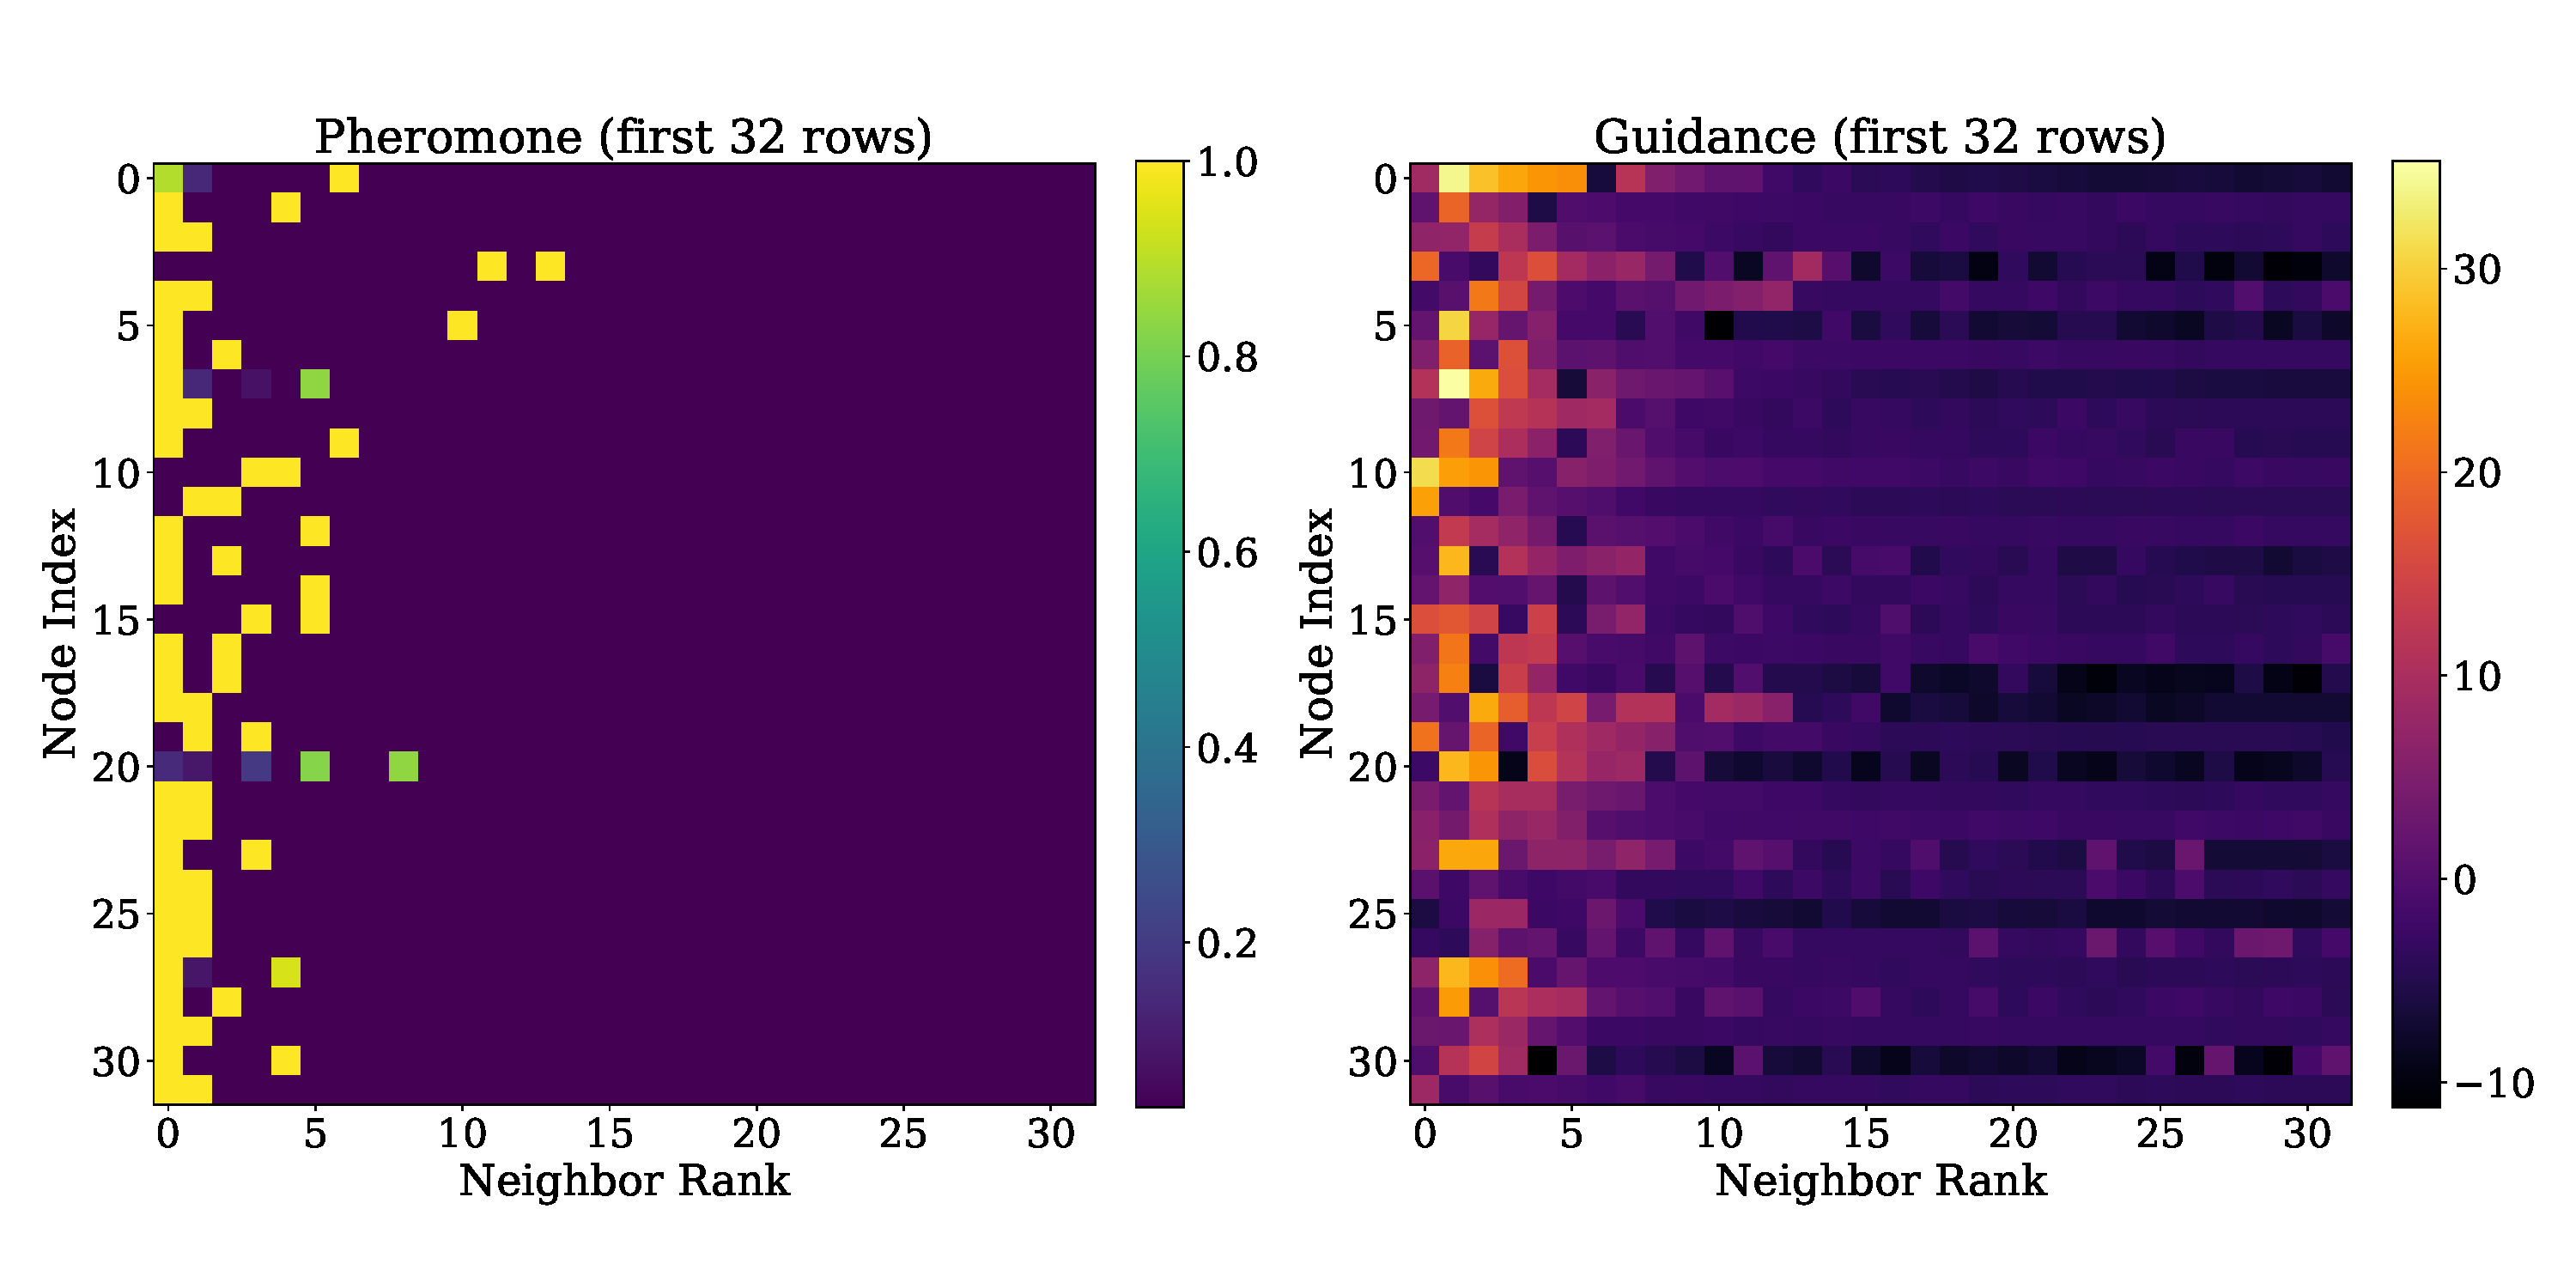
\includegraphics[width=\columnwidth]{figures/matrix_model_t5.pdf}
    \caption{Visualization of pheromone concentration and neural guidance scores (first 32 rows of the edge matrix) at successive iterations~$T$.}
    \label{fig:matrix_model}
\end{figure}

\smallskip\noindent\textbf{The policy learns to counteract ACO stagnation.}
Figure~\ref{fig:matrix_model} displays the pheromone matrix and corresponding neural guidance scores at successive iterations. As the search progresses, pheromone concentrations saturate and many edges converge toward $\tau_{\max}$, making the pheromone signal less informative. Despite this, the model outputs diverse guidance scores. In particular, over-reinforced edges often receive negative guidance, which redirects exploration away from stagnant regions. This selective counter-pressure is unavailable to static priors because they cannot observe the evolving pheromone landscape.

\smallskip\noindent\textbf{The 1K-trained model transfers zero-shot to larger synthetic scales.}
Table~\ref{tab:cross-scale} compares an in-scale model with the 1K-trained model on larger synthetic instances. The 1K model remains close to the in-scale model in all columns and is slightly better in two \TSP{}5K settings, providing scale-transfer evidence from a single trained policy.

\begin{table}[h]
\centering
\caption{Cross-scale zero-shot transfer: 1K model evaluated on larger instances.}
\label{tab:cross-scale}
\small
\renewcommand{\arraystretch}{0.80}
\begin{tabular*}{\columnwidth}{@{\extracolsep{\fill}}llcccc@{}}
\toprule
& & \multicolumn{2}{c}{$I_{1000}$} & \multicolumn{2}{c}{$I_{10000}$} \\
\cmidrule(lr){3-4} \cmidrule(lr){5-6}
Problem & Model & Gap & $\Delta$ & Gap & $\Delta$ \\
\midrule
\multirow{2}{*}{\TSP{}5K}
  & In-scale  & 1.30\% & --       & 0.75\% & --       \\
  & 1K model  & \textbf{1.23\%} & $-$0.07  & \textbf{0.72\%} & $-$0.03  \\
\midrule
\multirow{2}{*}{\TSP{}10K}
  & In-scale  & \textbf{1.59\%} & --       & \textbf{0.82\%} & --       \\
  & 1K model  & 1.66\% & +0.07    & 0.90\% & +0.08    \\
\midrule
\multirow{2}{*}{\CVRP{}5K}
  & In-scale  & \textbf{6.89\%} & --       & \textbf{3.36\%} & --       \\
  & 1K model  & 7.10\% & +0.21    & 3.60\% & +0.24    \\
\midrule
\multirow{2}{*}{\CVRP{}10K}
  & In-scale  & \textbf{11.04\%} & --      & \textbf{6.04\%} & --       \\
  & 1K model  & 11.72\% & +0.68   & 6.07\% & +0.03    \\
\bottomrule
\end{tabular*}
\end{table}

% \smallskip\noindent\textbf{\DyNACS{} generalizes zero-shot to real-world benchmarks.}
% Table~\ref{tab:realworld} evaluates the 1K-trained model on large TSPLIB and CVRPLIB instances without any fine-tuning. These instances include non-uniform, clustered, and geographically derived node distributions that differ substantially from the uniform training data. \DyNACS{} solves all instances and consistently improves over the unguided backend, confirming that the full guidance mechanism trained only on synthetic 1K instances can transfer to realistic benchmark distributions.

% \begin{table}[h]
% \centering
% \caption{Real-world benchmark results (zero-shot from 1K model, $I_{10000}$).}
% \label{tab:realworld}
% \small
% \renewcommand{\arraystretch}{0.80}
% \begin{tabular*}{\columnwidth}{@{\extracolsep{\fill}}lcccc@{}}
% \toprule
% & \multicolumn{2}{c}{TSPLIB (33)} & \multicolumn{2}{c}{CVRPlib (14)} \\
% \cmidrule(lr){2-3} \cmidrule(lr){4-5}
% Method & Gap (\%) & Time & Gap (\%) & Time \\
% \midrule
% LKH3 & 0.07 & 35m & 13.6 & 2.1h \\
% HGS & -- & -- & 5.15 & 5h \\
% \midrule
% LEHD~\cite{lehd}  & 13.2 & 38m & 16.9 & 40m \\
% GLOP~\cite{glop} & 6.99 & 34s & 20.6 & 39s \\
% SIL~\cite{sil} & 3.03 & 45m & 7.69 & 54m \\
% \midrule
% % ACO                   & 1.29 & 13s & 4.26 & 50.85s \\
% \textbf{\DyNACS{} (ours)}       & \textbf{0.89} & 11.57s & \textbf{3.66} & 51.07s \\
% \bottomrule
% \end{tabular*}
% \end{table}

\smallskip\noindent\textbf{Guidance--pheromone dynamics are consistent across scales.}
Figure~\ref{fig:guidance_pheromone_dynamics} shows a consistent two-phase interaction between neural guidance and pheromone. Early in the search, the policy tends to cooperate with pheromone by amplifying promising signals. Later, as pheromone concentrates and risks premature convergence, the policy increasingly suppresses over-reinforced edges to preserve exploration. The volatility diagnostics further show that guidance changes sharply after the first pheromone feedback, then settles into smaller but persistent updates across later outer steps. This rapid adaptation followed by steady refinement is expected from a policy that observes the search state directly: it reacts strongly when the pheromone field first becomes informative, then continues to recalibrate as the field evolves.

\begin{figure}[h]
    \centering

    \subfloat[Training correlation\label{fig:guidance_eta_corr}]{%
        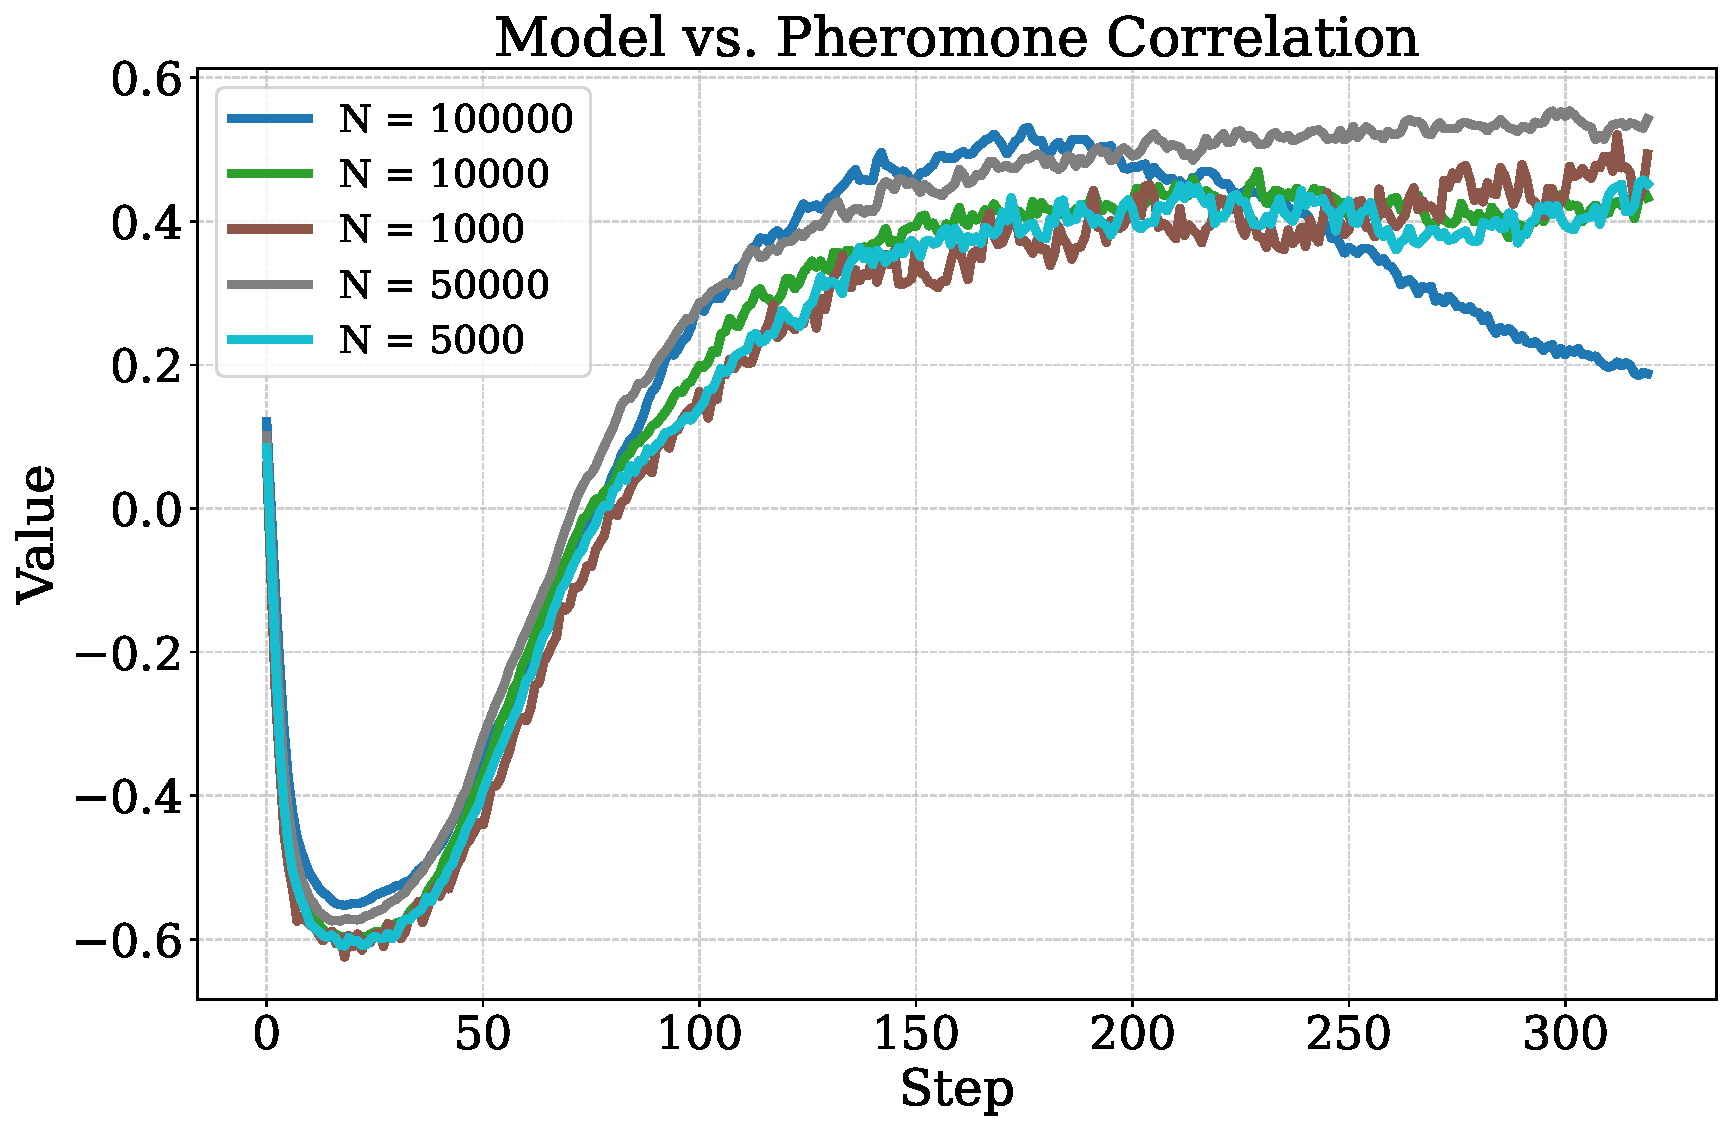
\includegraphics[width=.49\columnwidth]{figures/prior_eta_corr.pdf}%
    }
    \subfloat[Testing interaction\label{fig:interaction}]{%
        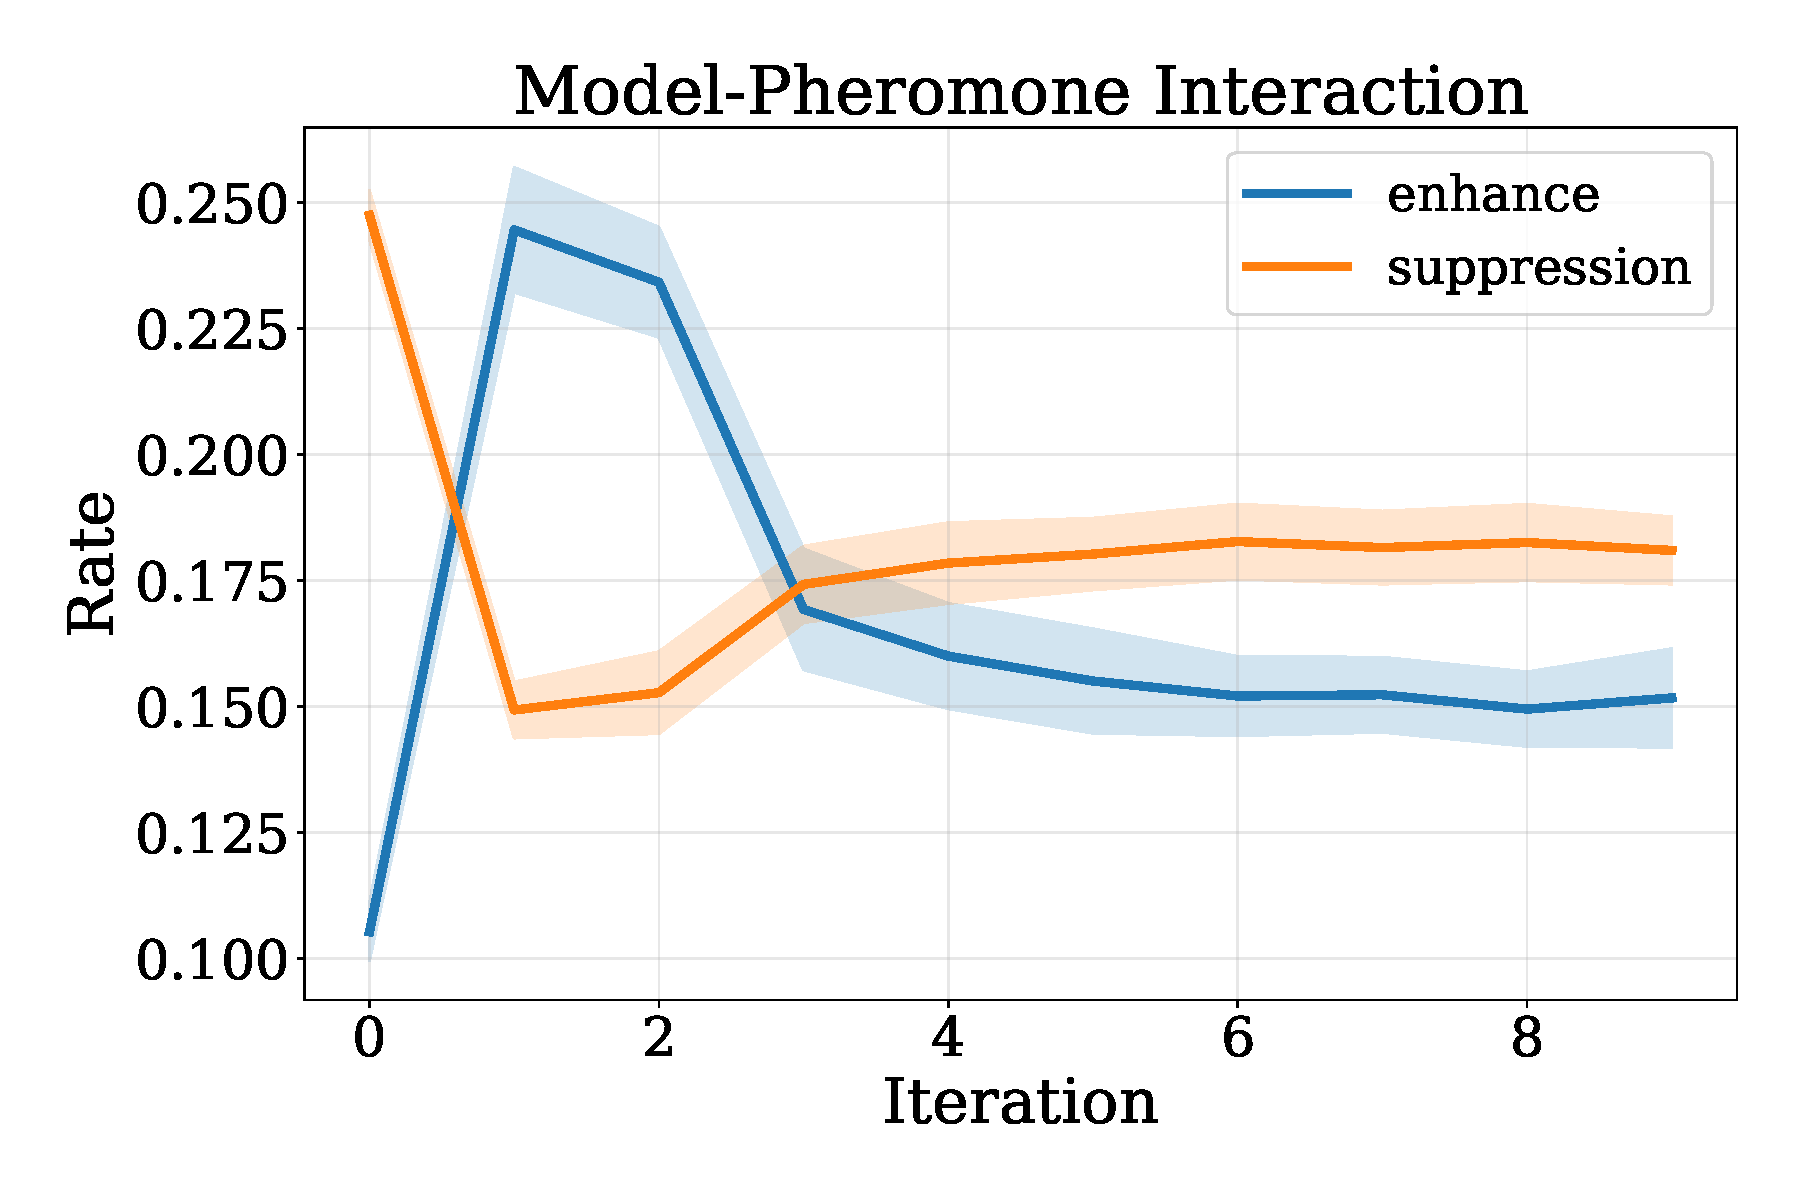
\includegraphics[width=.49\columnwidth]{figures/interaction.pdf}%
    }\hfill
    \subfloat[Guidance volatility\label{fig:prior_changes}]{%
        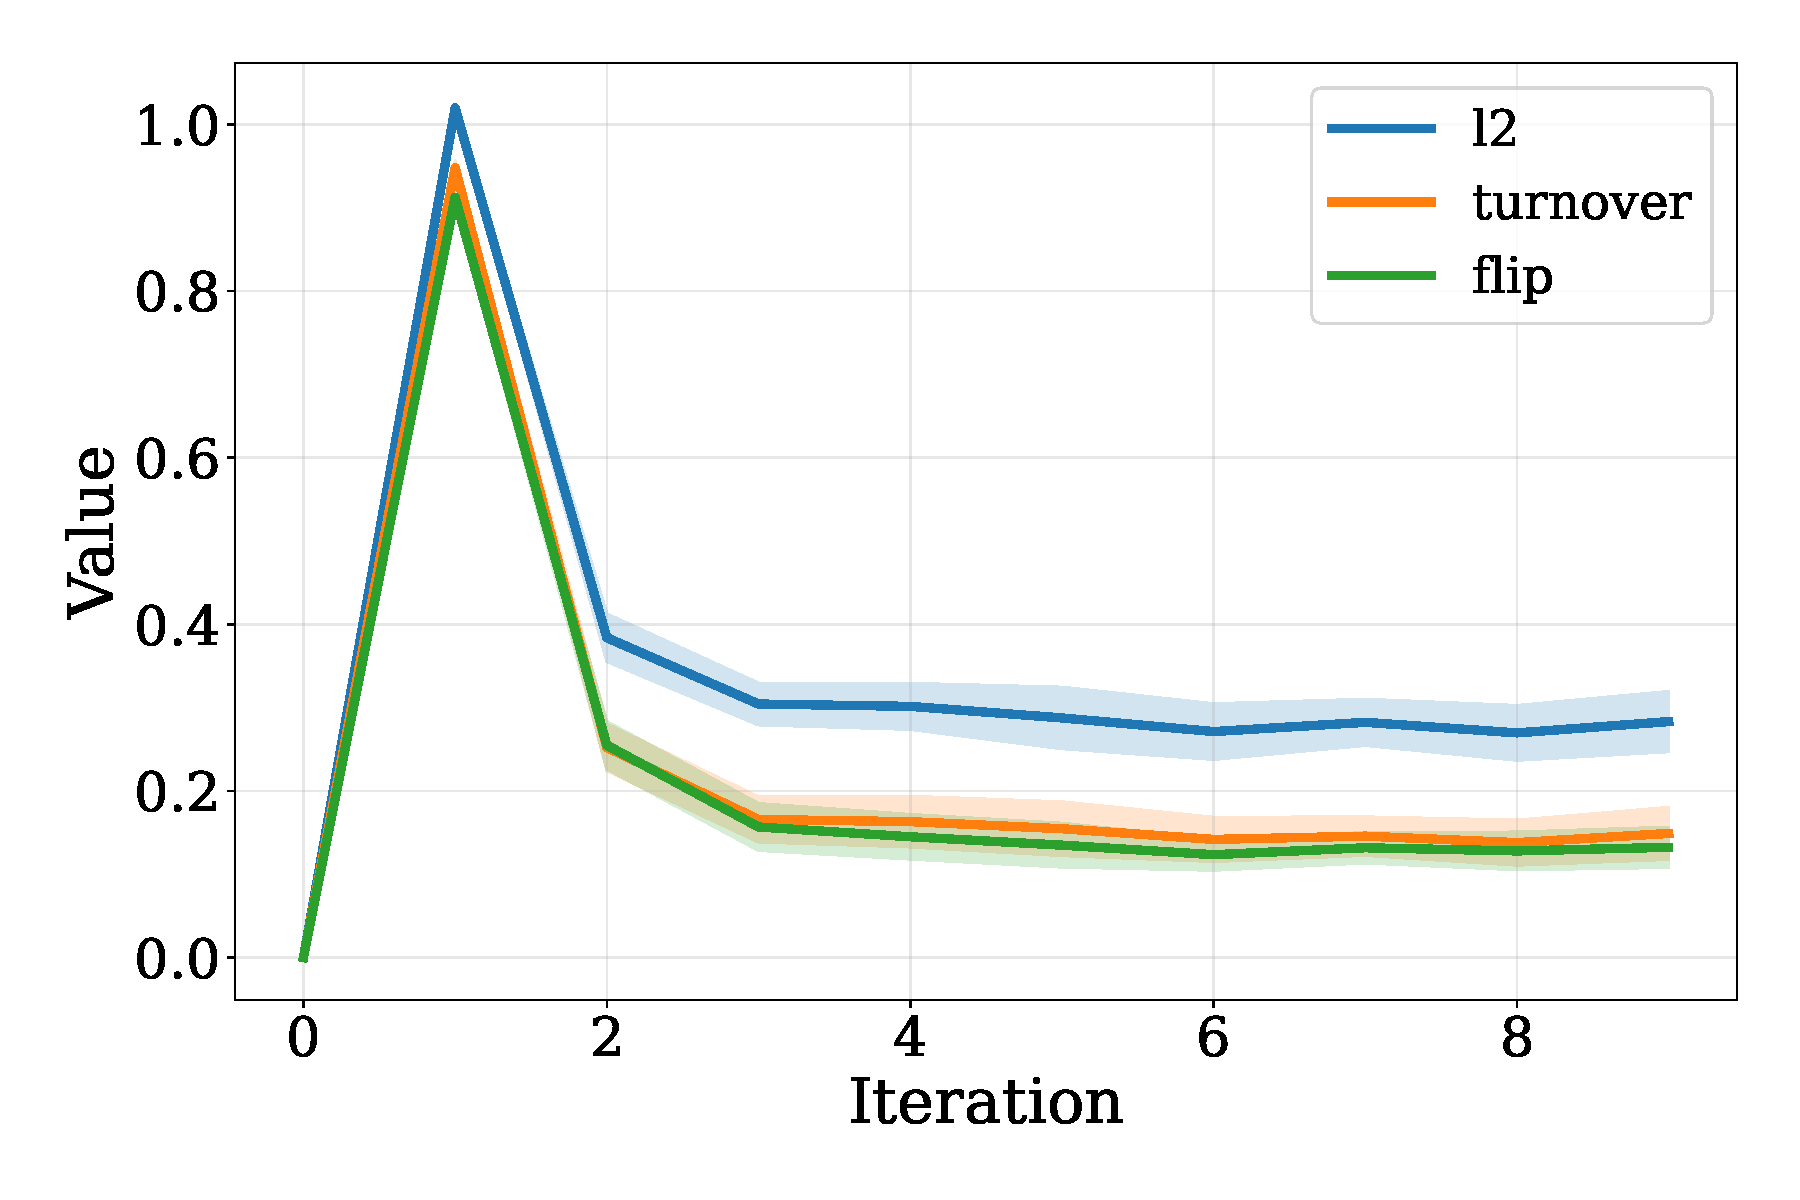
\includegraphics[width=.49\columnwidth]{figures/prior_changes.pdf}%
    }\hfill

    \caption{Visualization of the guidance-pheromone dynamics during both training and inference.}
    \label{fig:guidance_pheromone_dynamics}
\end{figure}


% ======================================================================
% Conclusion
% ======================================================================
\section{Conclusion}
\label{sec:conclusion}

We presented \DyNACS{}, a dynamic neural ant colony search model that builds trajectory-diverse guidance on top of \DyNACO{}. Neural guidance remains useful throughout an iterative ACO trajectory when it observes the evolving search state and supports multiple complementary search behaviors. Across \TSP{} and \CVRP{} benchmarks, \DyNACS{} improves over the unguided backend and prior neural baselines while preserving the scalability needed for large routing instances.

One limitation is that the macro step granularity $(H,S)$ and the $K$-NN candidate graph require problem-specific configuration, and models are currently trained at a fixed scale.
Future work includes: (1)~adaptive candidate selection to address the fixed-$K$ reachability constraint; (2)~adaptive macro step duration, e.g., changing $S$ based on stagnation while preserving the semi-MDP abstraction; (3)~curriculum or training across multiple scales, which must handle feature scale discrepancies and possible gradient conflicts across instance sizes and may require meta-learning or scale-normalized attention designs; and (4)~extending dynamic neural guidance to other combinatorial domains and metaheuristic families.

% ======================================================================
% Appendix
% ======================================================================
\appendix
\section{Details of Algorithms and Hyperparameters}
\label{app:setup}

This appendix collects implementation details that support the method sections: the routing backend instantiations, the local optimality property of SRR, and the default hyperparameters and sensitivity tables used in the experiments.

\subsection{Routing Backend Instantiation}
\label{app:backend}

Perturbation and local projection must keep feasibility handling and refinement local to the sampled intervention region, so each ant can receive a post-refinement reward without running full-scale local search. For \TSP{}, we follow~\cite{faco}: ants perform at most $M$ relocation steps starting from the incumbent $b$, with node selection governed by the shaped kernel $p^\theta$. Each ant touches at most $\mathcal{O}(M \cdot K)$ edges, where $M \ll N$ and $K{=}32$, independent of problem size.

\subsection{CVRP Feasibility Interface}
\label{app:cvrp}

For \CVRP{}, the perturbation backend must preserve route capacity while still allowing local changes around the policy-selected intervention. We maintain an explicit multi-route structure using linked lists, where each route $r$ tracks its current load $L_r$. Transitions to node $j$ are masked if $\mathrm{Load}+d_j>Q$. Same-route reordering is always feasible because it preserves load; cross-route insertion is feasible only if $L_{r_u}+d_v\le Q$; and depot targets trigger route splits and are always feasible. The new-edge counter tracks cross-route edges specifically, ensuring sufficient inter-route perturbation for effective local search. The policy follows the DeepACO feature convention for static node inputs, including demand/capacity features, while dynamic edge-state features are derived from pheromone and incumbent information.

The CVRP local projection phase applies four capacity-preserving operators restricted to the checklist of perturbed nodes: intra-route 2-opt, inter-route relocate, inter-route swap, and 2-opt* cross-route segment exchange. Each operator only evaluates moves involving checklist nodes and $K$-nearest candidate neighbors, and all moves must preserve route capacity. We use don't-look-bit optimization so that nodes are deactivated when no improving move is found and reactivated only when a neighbor participates in an accepted move.

\subsection{SRR Local Optimality}
\label{app:credit}

Let $\mathcal{B}^*$ be a 2-opt optimal incumbent. A policy perturbation replaces edges $E_{\mathrm{rem}}$ with $E_{\mathrm{add}}$, yielding $\mathcal{B}'$. Since only the neighborhood of $E_{\mathrm{add}}$ can become suboptimal, SRR initializes a checklist with the endpoints of the added edges and propagates improving moves outward until no checked node admits improvement. If SRR terminates with an empty checklist, the resulting tour $\mathcal{B}''$ is 2-opt optimal under the candidate-graph move set.

\begin{proof}
Let $\mathcal{C}$ be the set of edges modified by the perturbation or SRR\@. All edges outside $\mathcal{C}$ are unchanged from the 2-opt optimal incumbent $\mathcal{B}^*$, so no improving 2-opt move can use only those edges. SRR starts from all perturbed endpoints and reactivates affected nodes after each accepted move; hence an empty checklist certifies that no candidate-graph 2-opt move involving any edge in $\mathcal{C}$ is improving. Cross-boundary moves also involve an edge in $\mathcal{C}$ and are therefore covered. Thus no improving candidate-graph 2-opt move remains in $\mathcal{B}''$.
\end{proof}

\subsection{Hyperparameters}
\label{app:repro}

\begin{table}[t]
\centering
\caption{Default hyperparameters for \DyNACS{}.}
\label{tab:hyperparams}
\small
\renewcommand{\arraystretch}{0.85}
\begin{tabular*}{\columnwidth}{@{\extracolsep{\fill}}llc@{}}
\toprule
Category & Parameter & Value \\
\midrule
\multirow{4}{*}{ACO Backend}
    & Ants $m$ & 100 \\
    & Outer steps $H$ & 10 \\
    & Inner steps $S$ & 100 \\
    & New-edge steps $M$ & 12 \\
\midrule
\multirow{3}{*}{Pheromone}
    & Evaporation $\rho$ (TSP / CVRP) & 0.1 / 0.5 \\
    & $\tau_{\max}$ & 1.0 \\
    & $\tau_{\min}$ & $1/K$ \\
\midrule
\multirow{2}{*}{Graph}
    & $K$-NN candidates & 32 \\
    & Backup neighbors & 64 \\
\midrule
\multirow{5}{*}{PPO Training}
    & Learning rate & $5 \times 10^{-6}$ \\
    & PPO clip $\epsilon$ & 0.1 \\
    & PPO epochs $K_{\text{PPO}}$ & 4 \\
    & Optimizer & AdamW + cosine \\
    & Guidance weight $\gamma$ (train) & 1.0 \\
\midrule
\multirow{3}{*}{Architecture}
    & GNN layers $L$ & 12 \\
    & Hidden dimension $d$ & 32 \\
    & MLP decoder layers & 3 \\
\bottomrule
\end{tabular*}
\end{table}

We use a 12-layer GNN encoder~\cite{deepaco} with residual connections and batch normalization; the decoder is a 3-layer MLP projecting edge embeddings to scalar log-priors. With the three-channel edge representation, the policy has 67,265 parameters, compared with 67,201 parameters for the corresponding static-input variant. The parameter count is constant across problem scales because the architecture operates on local $K$-NN neighborhoods.

\subsection{State-Aware Edge Features}
\label{app:features}

For static node features, we follow~\cite{deepaco}, using node coordinates for \TSP{} and demand/capacity for \CVRP{}. The dynamic edge features are recomputed at every outer step from the current pheromone field and incumbent solution. With stabilized pheromone bounds $\tau_{\max}=1$ and $\tau_{\min}=1/K$, the representation has three edge channels and $\mathcal{O}(nK)$ size for fixed $K$.

\begin{table}[t]
\centering
\caption{Dynamic edge features used by the state-aware policy.}
\label{tab:state-features}
\small
\setlength{\tabcolsep}{3pt}
\renewcommand{\arraystretch}{0.95}
\begin{tabular*}{\columnwidth}{@{}c@{\extracolsep{\fill}}p{0.39\columnwidth}p{0.42\columnwidth}@{}}
\toprule
Feature & Definition & Meaning \\
\midrule
$f_1$ & $d_{ij}/\bar d_i$ & Scale-normalized distance. \\
$f_2$ & $\log(\tau_{ij}/\bar\tau_i)$ & Edge pheromone relative to other candidates of $i$. \\
$f_3$ & $\mathbf{1}[j\notin\{\mathrm{succ}_b(i),\mathrm{pred}_b(i)\}]$ & Edge that introduces new tour structure. \\
\bottomrule
\end{tabular*}
\end{table}

\subsection{Detailed Sensitivity and Memory Tables}
\label{extended_ablation}

Table~\ref{tab:ablation-mmas-app} examines pheromone bound strategies. Standard \MMAS{} couples bounds to solution cost, creating non-stationary dynamics. Our stabilized variant ($\tau_{\max}{=}1$, $\tau_{\min}{=}1/K$) yields scale-invariant state representations and reduced training variance.

\begin{table}[t]
\centering
\caption{Environment stabilization. We report results without inference strategies.}
\label{tab:ablation-mmas-app}
\small
\renewcommand{\arraystretch}{0.85}
\begin{tabular*}{\columnwidth}{@{\extracolsep{\fill}}lcc@{}}
\toprule
Bound Strategy & Obj. & Gap (\%)\\
\midrule
ACO (Standard \MMAS{}) & 51.8318 & 1.68  \\
ACO (Stabilized) & 52.0747 & 2.16 \\
\DyNACO{} (Standard \MMAS{}) & 51.7022 & 1.43 \\
\DyNACO{} (Stabilized) & 51.6795 & 1.38 \\
\bottomrule
\end{tabular*}
\end{table}

\begin{table*}[t]
\centering
\caption{Sensitivity to outer guidance updates $H$ and inner ACO steps $S$.}
\label{tab:hs-sensitivity-app}
\small
\renewcommand{\arraystretch}{0.85}
\begin{tabular*}{\textwidth}{@{\extracolsep{\fill}}llcccccccc@{}}
\toprule
$H$ & $S$ & TSP-1K Obj. & Time & TSP-5K & Time & CVRP-1K & Time & CVRP-5K & Time \\
\midrule
5 & 200 & 23.22 & 0.32 & 51.59 & 0.75 & 36.62 & 1.34 & \textbf{96.16} & 3.07 \\
10 & 100 & 23.23 & \textbf{0.32} & 51.63 & \textbf{0.76} & \textbf{36.28} & \textbf{1.27} & 96.81 & \textbf{2.73} \\
20 & 50 & \textbf{23.21} & 0.42 & \textbf{51.56} & 0.87 & 36.49 & 1.33 & 97.17 & 2.82 \\
\bottomrule
\end{tabular*}
\end{table*}

Table~\ref{tab:memory-scaling} reports peak GPU memory usage for representative constructive and neural-ACO baselines. Methods based on dense attention or dense heatmaps scale quadratically in the number of nodes and become infeasible at larger scales. \DyNACO{} instead operates on a fixed-size sparse candidate graph and uses perturbation-based sampling, so memory scales approximately linearly with $n$ for fixed $K$.

\begin{table}[t]
\centering
\caption{Peak GPU memory usage (GB) on TSP instances. OOM: out of memory.}
\label{tab:memory-scaling}
\small
\renewcommand{\arraystretch}{0.85}
\begin{tabular*}{\columnwidth}{@{\extracolsep{\fill}}lccccc@{}}
\toprule
Method & 1K & 5K & 10K & 50K & 100K \\
\midrule
POMO & 0.10 & 2.54 & 10.11 & OOM & OOM \\
SIGD & 0.04 & 0.95 & 3.76 & OOM & OOM \\
LEHD & 0.10 & 2.27 & 9.01 & OOM & OOM \\
DeepACO & 0.14 & 2.11 & 8.31 & OOM & OOM \\
\DyNACO{} & \textbf{0.08} & \textbf{0.18} & \textbf{0.35} & 1.57 & 3.11 \\
\bottomrule
\end{tabular*}
\end{table}

Table~\ref{tab:k-sensitivity-app} and Table~\ref{tab:m-sensitivity-app} evaluate the candidate-graph size $K$ and perturbation length $M$.

\begin{table}[t]
\centering
\caption{Sensitivity to candidate-graph size $K$.}
\label{tab:k-sensitivity-app}
\small
\renewcommand{\arraystretch}{0.85}
\begin{tabular*}{\columnwidth}{@{\extracolsep{\fill}}lcccc@{}}
\toprule
$K$ & TSP-5K & Time & CVRP-5K & Time \\
\midrule
32 & 51.63 & \textbf{0.76} & 96.81 & \textbf{2.73} \\
48 & 51.49 & 0.98 & 95.83 & 3.51 \\
64 & \textbf{51.47} & 1.17 & \textbf{95.08} & 4.42 \\
\bottomrule
\end{tabular*}
\end{table}

\begin{table}[t]
\centering
\caption{Sensitivity to perturbation length $M$.}
\label{tab:m-sensitivity-app}
\small
\renewcommand{\arraystretch}{0.85}
\begin{tabular*}{\columnwidth}{@{\extracolsep{\fill}}lcccc@{}}
\toprule
$M$ & TSP-5K & Time & CVRP-5K & Time \\
\midrule
8 & \textbf{51.62} & \textbf{0.73} & 97.13 & \textbf{2.37} \\
12 & 51.63 & 0.76 & 96.81 & 2.73 \\
16 & 51.77 & 0.82 & \textbf{96.48} & 3.24 \\
\bottomrule
\end{tabular*}
\end{table}

\DyNACO{} adds dynamic state features to a compact GNN policy. The peak GPU-memory overhead of these additional features remains small even at 100K nodes, as shown in Table~\ref{tab:feature-memory-app}.

\begin{table}[t]
\centering
\caption{Peak GPU memory (GB) for static and dynamic policy inputs.}
\label{tab:feature-memory-app}
\small
\renewcommand{\arraystretch}{0.85}
\begin{tabular*}{\columnwidth}{@{\extracolsep{\fill}}llcc@{}}
\toprule
Problem & Scale & Static (GB) & Dynamic (GB) \\
\midrule
TSP & 10K & 0.286 & 0.293 \\
TSP & 100K & 2.524 & 2.584 \\
CVRP & 10K & 0.286 & 0.292 \\
CVRP & 100K & 2.513 & 2.573 \\
\bottomrule
\end{tabular*}
\end{table}

% ======================================================================
% Acknowledgments
% ======================================================================
% \section*{Acknowledgments}
% Lorem ipsum dolor sit amet, consectetur adipiscing elit. Cras vitae fermentum est. Donec lobortis facilisis augue, id commodo libero vulputate vel. Cras dictum velit et lectus pellentesque vulputate. 

% ======================================================================

\section*{Data and Code Availability}
The source code, datasets, and pretrained model checkpoints associated with this work are publicly available at \url{https://doi.org/10.5281/zenodo.20502184}. The implementation repository is available at \url{https://github.com/shoraaa/DyNACO}.

% Add an acknowledgment section here when funding or contributor information is available.
% \section*{Acknowledgment}

\bibliographystyle{IEEEtran}
\bibliography{references}

% Optional author biographies may be added using IEEEbiography environments.

\end{document}
